\chapter{СБОРКА И ТЕСТИРОВАНИЕ ГЕНЕРАТОРА СИГНАЛОВ}
\section{Конструирование макета}
	По структурной схеме (рис. 2.7) создадим схему электрическую принципиальную. 
	
	\begin{figure}[H]
    \centering
    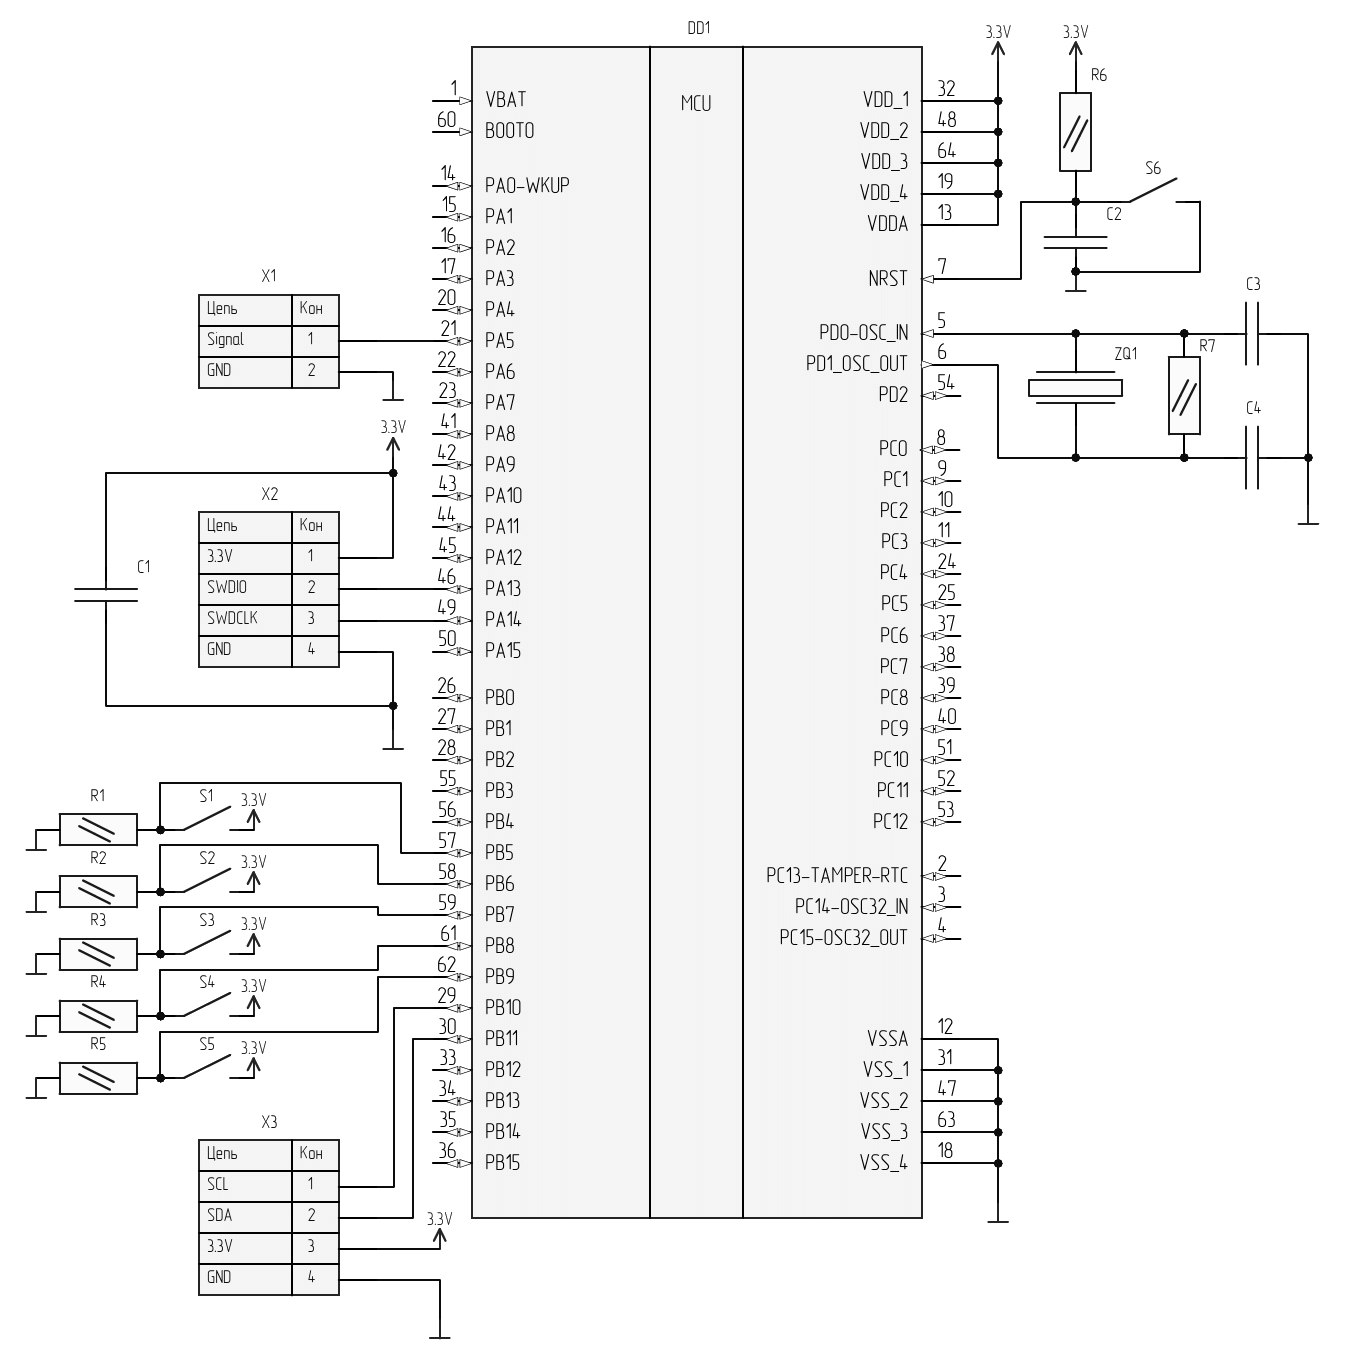
\includegraphics[width=1\textwidth]{../image/scheme-cropped.png}
    \caption{Схема электрическая принципиальная.}
	\end{figure}
	
	Просто так контроллер работать не сможет. Необходим внешний кварцевый резонатор для стабилизации частоты системного тактового генератора, а также функция сброса. Эти узлы уже реализованы на отладочной плате микроконтроллера. Питание схемы будет подаваться через разъём SWD.
		
	Для улучшения генерации будет задействован встроенный в цифро-аналоговый преобразователь выходной буфер. При его использовании он будет срезать сигнал сверху и снизу на 0.2В, поэтому значения тоже следует срезать на эту же величину для корректной генерации.
	
	В документе от STM про работу с цифро-аналоговым преобразователем есть формула для расчета выходного напряжения~\cite{an3126}.
	
	\begin{gather}
	DAC_{output} = V_{REF}*\dfrac{DOR}{DAC_{MaxDigitalValue} + 1},
	\end{gather}
	
	где $DAC_{output}$ --- выходное напряжение ЦАП,
	
	$V_{REF}$ --- опорное напряжение,
	
	$DOR$ --- цифровое значение выходного напряжения,
	
	$DAC_{MaxDigitalValue}$ --- максимальное значение $DOR$.
	
	Нам нужно найти какое значение соответствует напряжению 0.2В. Выразим DOR и подставим имеющиеся значения.
	
	\begin{center}
	$DOR = \dfrac{V_{REF}}{DAC_{output}}*DAC_{MaxDigitalValue} + 1 = \dfrac{3.3}{0.2}*(4095+1) = 248$
	\end{center}
	
	Поэтому для отсчётов нужно будет указать смещение от нуля 248, а максимальное значение 4095 меньше на 248, то есть 3847. 
	
	Для управления потребуется 5 кнопок
	\begin{enumerate}
		\item Уменьшить частоту.
		\item Увеличить частоту.
		\item Предыдущий сигнал.
		\item Следующий сигнал.
		\item Выбор шага.
	\end{enumerate}
	
	Выделим для кнопок выводы PB5 - PB9. Постоянно быть подключенными к напряжению или земле выводы не могут, т. к. не будет возможности подавать на них какой-либо информационный сигнал. На выводы могут наводиться произвольные потенциалы, что негативно влияет на работу схемы. Подобные потенциалы имитируют сигналы, которые не предусмотрены. Из-за них может нарушиться логика работы, поэтому их принято фиксировать~\cite{schemat}. 
	
	Для этого используют подтягивающие (Pull - up) или заземляющие (Pull - down) резисторы. Они создают цепь, которая обеспечивает подтяжку сигнала к напряжению питания или земле. Если резисторы имеют большие сопротивления, то сигналы относят к слабым. При подключении сильных информационных сигналов происходит преодоление слабых и функциональность схемы не нарушается~\cite{butres}.
	
	\begin{figure}[H]
    \centering
    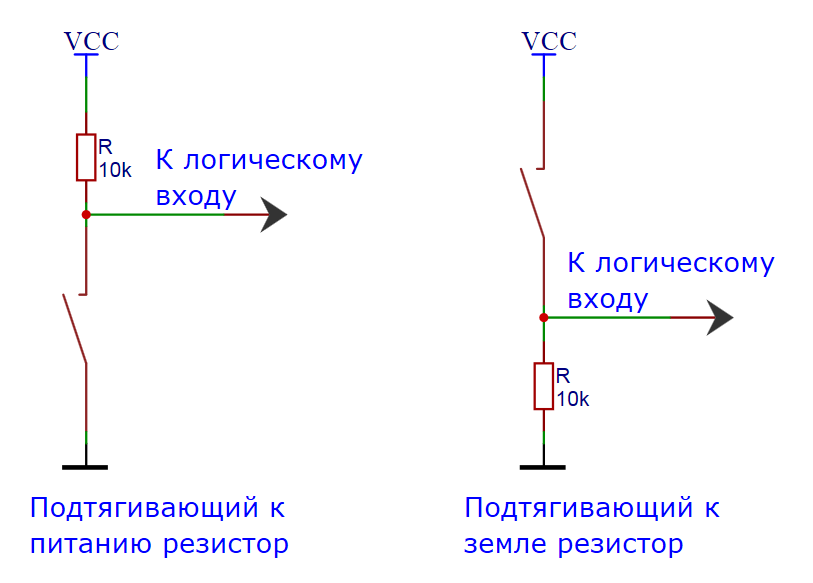
\includegraphics[width=0.55\textwidth]{../image/res.png}
    \caption{Pull-up и Pull - down резисторы.}
	\end{figure}
	
	В схеме устройства будет использоваться подтяжка к земле для считывания высокого уровня сигнала, то есть будет использоваться прямая логика. Рассчитаем минимальное и максимальное сопротивление заземляющего резистора.
	\begin{gather}
	R_{min} = \dfrac{V_{0}}{I_{max}},
	\end{gather}
	
	где $V_{0}$ --- напряжение логического нуля,
	
	$I_{max}$ --- максимальный ток вывода.
	
	Согласно спецификации микроконтроллера напряжение логического нуля составляет 1,16 В, а максимальный протекающий ток через пин может быть 25 мА~\cite{f103}. 
	
\begin{center}
	$R_{min} = \dfrac{1,16}{25*10^{-3}} = 46,4$ Ом.
\end{center}

	Для расчета максимального сопротивления формула следующая:
	\begin{gather}
	R_{max} = \dfrac{t}{C_{I/O}},
	\end{gather}
	
	где $t$ --- время нарастания сигнала,
	
	$C_{I/O}$ --- ёмкость вывода.
	
	Ёмкость вывода составляет 5 пФ, время нарастания возьмём 1 микросекунду (стандартный сигнал 100 кГц).
	
\begin{center}
	$R_{max} = \dfrac{1*10^{-6}}{5*10^{-12}} = 200$ кОм.
\end{center}	

	Из расчётов можно сделать вывод, что номинал резистора расположен в следующих границах.
	
\begin{center}
	$46,4$ Ом$ < R < 200$ кОм.
\end{center}	

	Разброс довольно большой, но из практики известно, что подтягивающий резистор имеет номинал 1 - 10 кОм.
	
	Для отображения информации будет использоваться дисплей, работающий по интерфейсу I2C.	
	
	Данный интерфейс широко применяется в микропроцессорных системах и его достоинство состоит в том, что передача данных идёт всего через две линии~\cite{schemat}. Одна линия для информации (SDA), вторая для синхросигнала (SCL). Для них также используются подтягивающие резисторы.
	
	\begin{figure}[H]
    \centering
    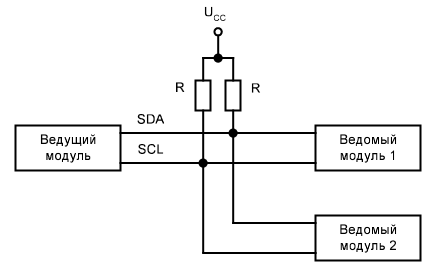
\includegraphics[width=0.525\textwidth]{../image/i2c.png}
    \caption{Организация интерфейса.}
	\end{figure}
	
	Интерфейс в микроконтроллере расположен на выводах PB10 (SCL) и PB11 (SDA). Также для дисплея потребуется питание 3.3 В.
	
	Дисплей и кнопки расположим на макетной плате размером 50 на 50 мм.
	
	\begin{figure}[H]
    \centering
    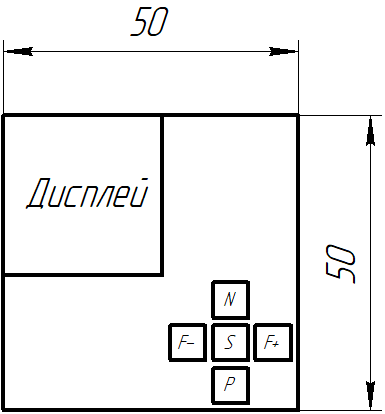
\includegraphics[width=0.45\textwidth]{../image/func_gen.png}
    \caption{Расположение периферии.}
	\end{figure}
	
	Назначения кнопок:
	\begin{enumerate}
	\item F- --- уменьшить частоту.
	\item F+ --- увеличить частоту.
	\item P --- предыдущий сигнал.
	\item N --- следующий сигнал.
	\item S --- переключить шаг по частоте.
	\end{enumerate}
	
	В результате сборки получилась плата с периферией.

	\begin{figure}[H]
    \centering
    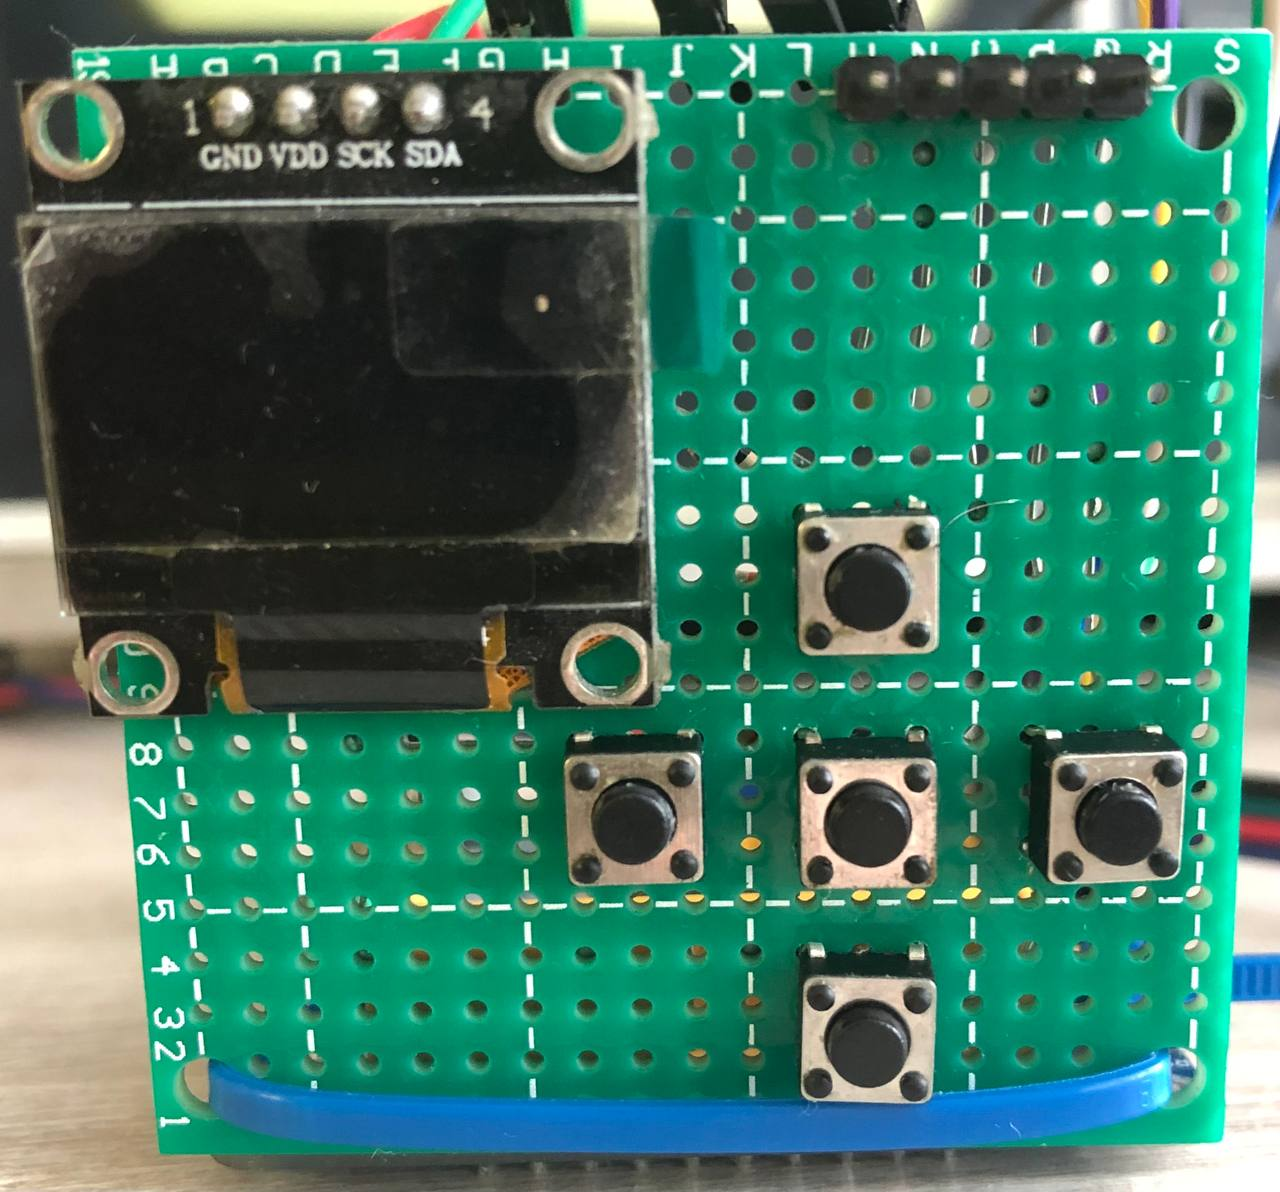
\includegraphics[width=0.5\textwidth]{../image/m1.jpeg}
    \caption{Плата периферии.}
	\end{figure}	
	
	Макет устройства будет состоять из отладочной платы микроконтроллера и полученной платы периферии. Обе части будут соединены проводами. Выход цифро-аналогового преобразователя, на котором генерируется сигнал, расположен на отладочной плате. В результате конструирования получился следующий макет устройства (рис. 3.6).

	\begin{figure}[H]
    \centering
    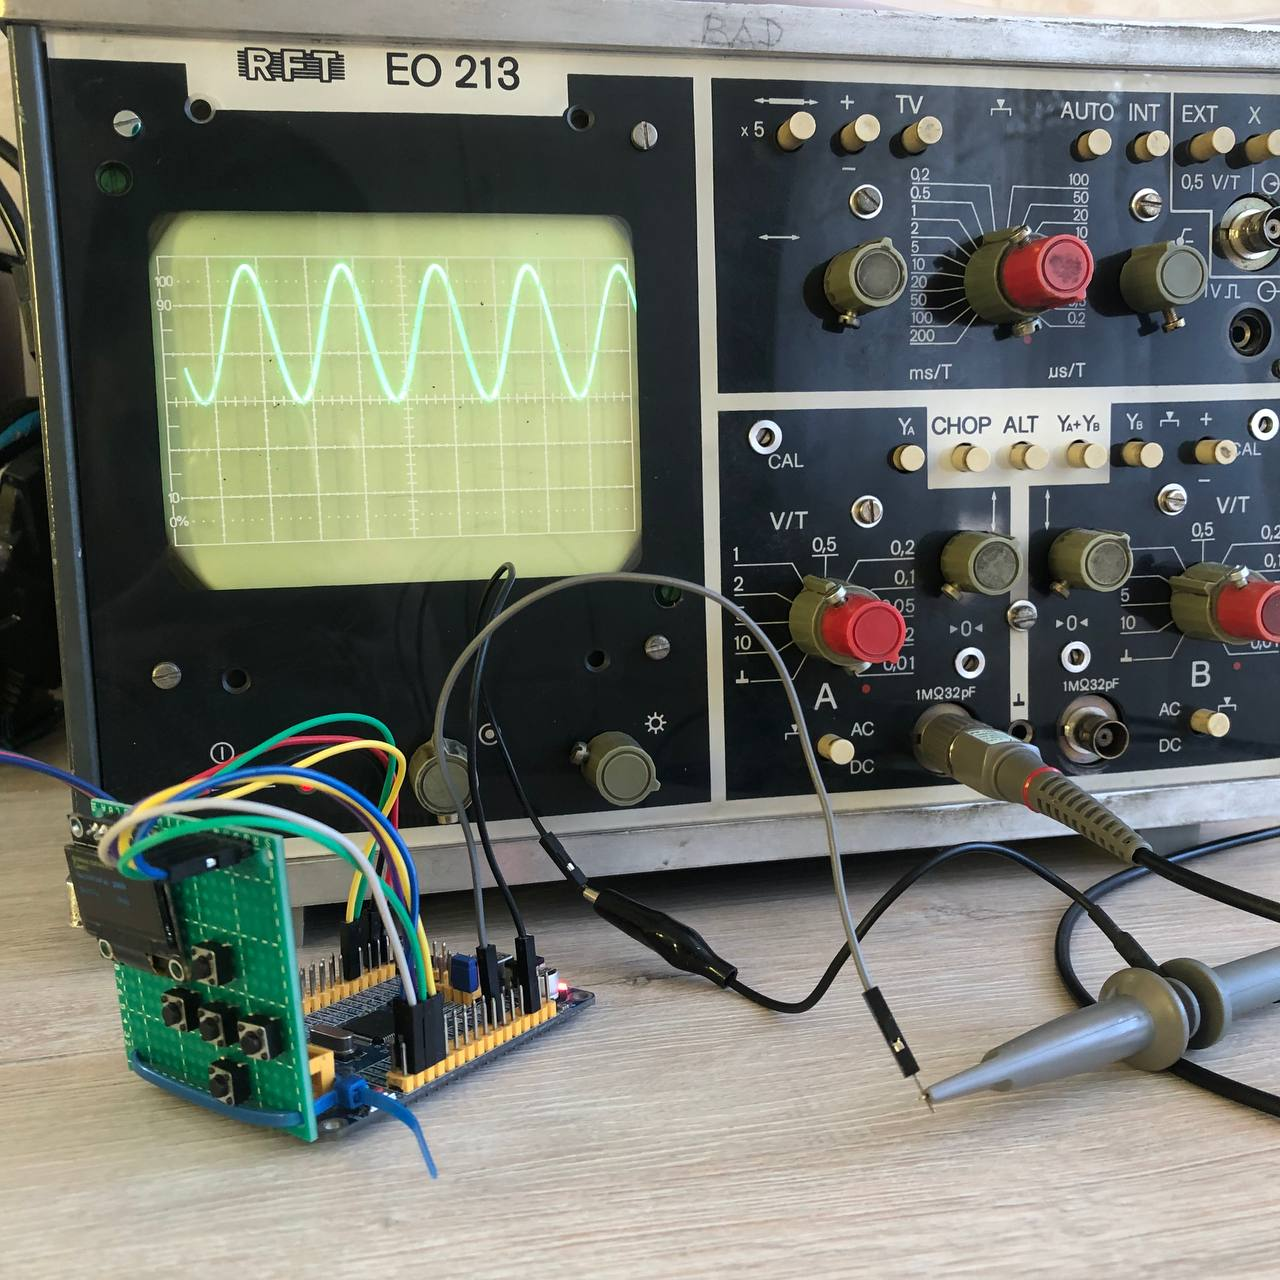
\includegraphics[width=0.5\textwidth]{../image/m2.jpg}
    \caption{Макет устройства.}
	\end{figure}	

\section{Тестирование устройства}
	
	После запуска устройства на экране появляются строки с пустыми параметрами формы сигнала, частоты и шага.

	\begin{figure}[H]
     \begin{subfigure}[H]{0.5\textwidth}
         \centering
         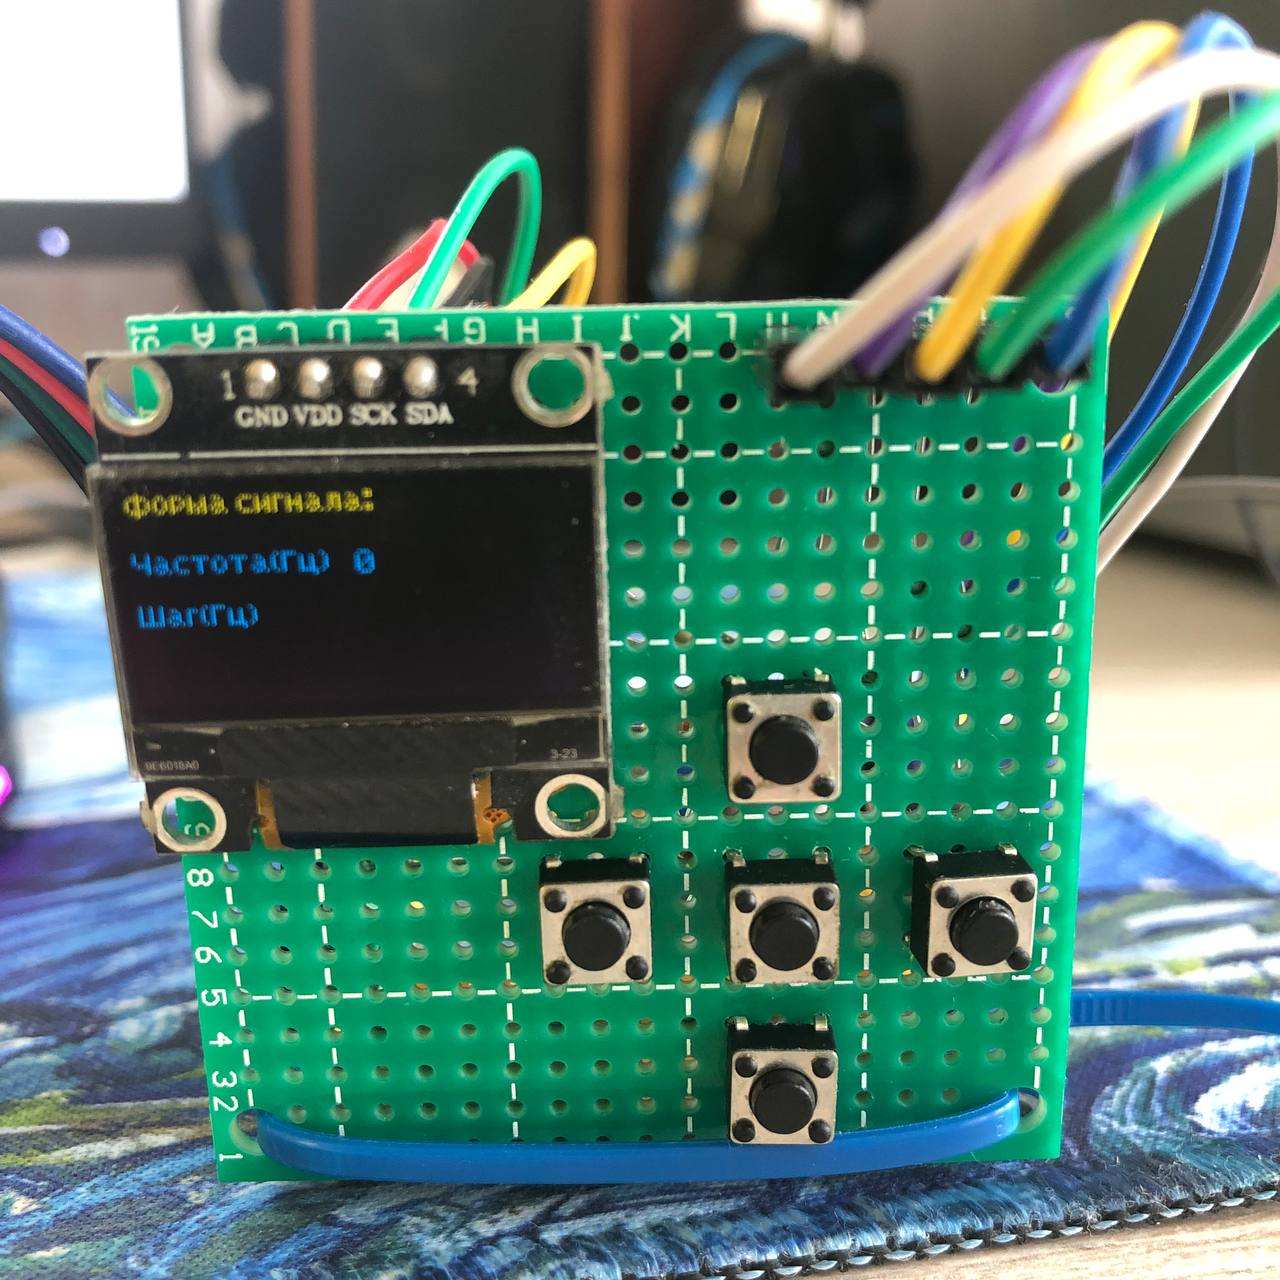
\includegraphics[width=0.8\textwidth]{../image/test0_u_s.jpg}
         \caption{Устройство.}
     \end{subfigure}
     \hfill
     \begin{subfigure}[H]{0.5\textwidth}
         \centering
         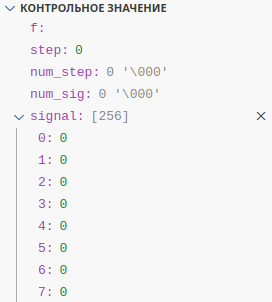
\includegraphics[width=0.7\textwidth]{../image/test0_o_s.png}
         \caption{Отладчик.}
     \end{subfigure}
        \caption{Начальное состояние.}
	\end{figure}
	
	Логика работы дисплея описана блок-схемой (рис. 3.8).
	
	\begin{figure}[H]
    \centering
    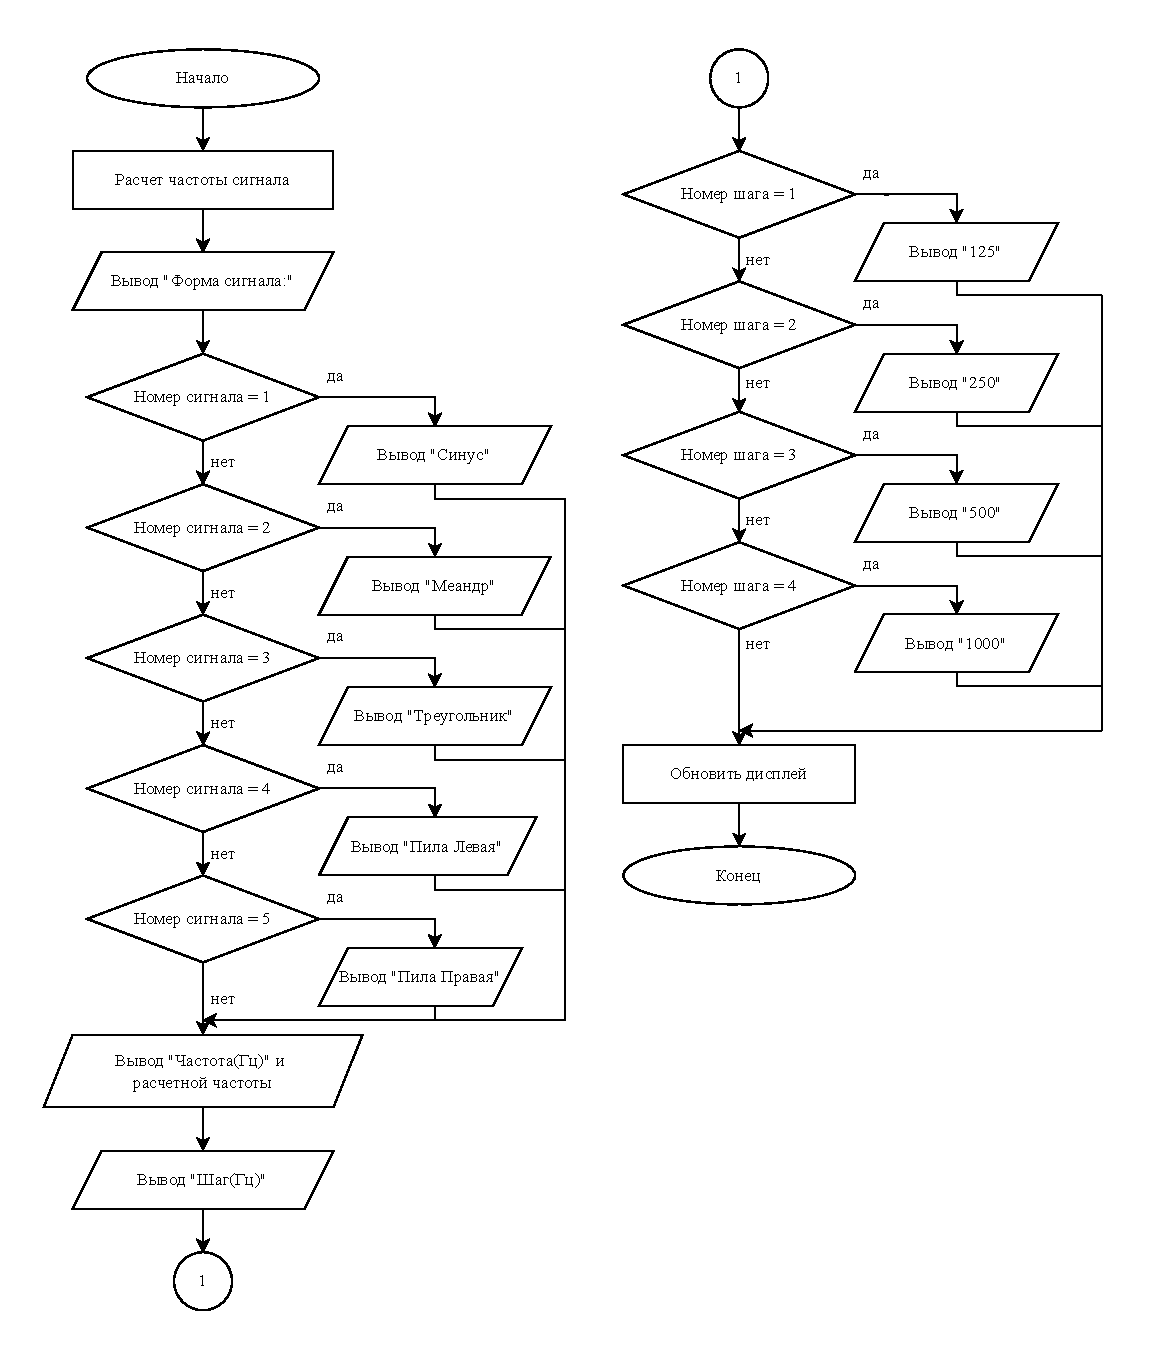
\includegraphics[width=1\textwidth]{../image/display.pdf}
    \caption{Алгоритм дисплея.}
	\end{figure}	
	
	Требуется выставить параметры сигнала. Клавишами N и P выбирается форма сигнала. При нажатии клавиши N выполняется алгоритм, описанный блок-схемой (рис. 3.10).
	
	\begin{figure}[H]
    \centering
    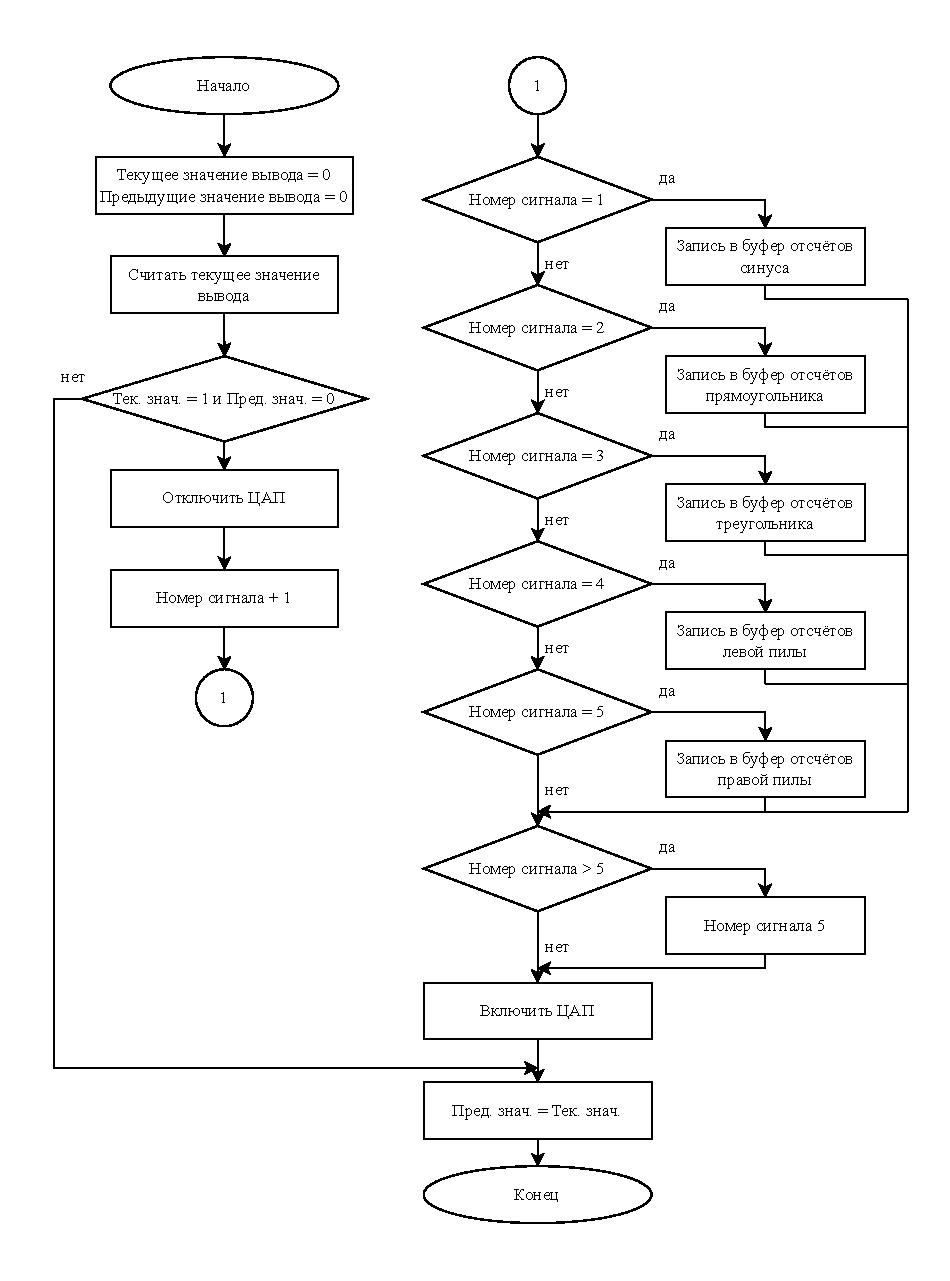
\includegraphics[width=1\textwidth]{../image/plus_signal.pdf}
    \caption{Выбор следующего сигнала.}
	\end{figure}	
	
	Просмотрим сигналы.
	\begin{figure}[H]
     \begin{subfigure}[H]{0.5\textwidth}
         \centering
         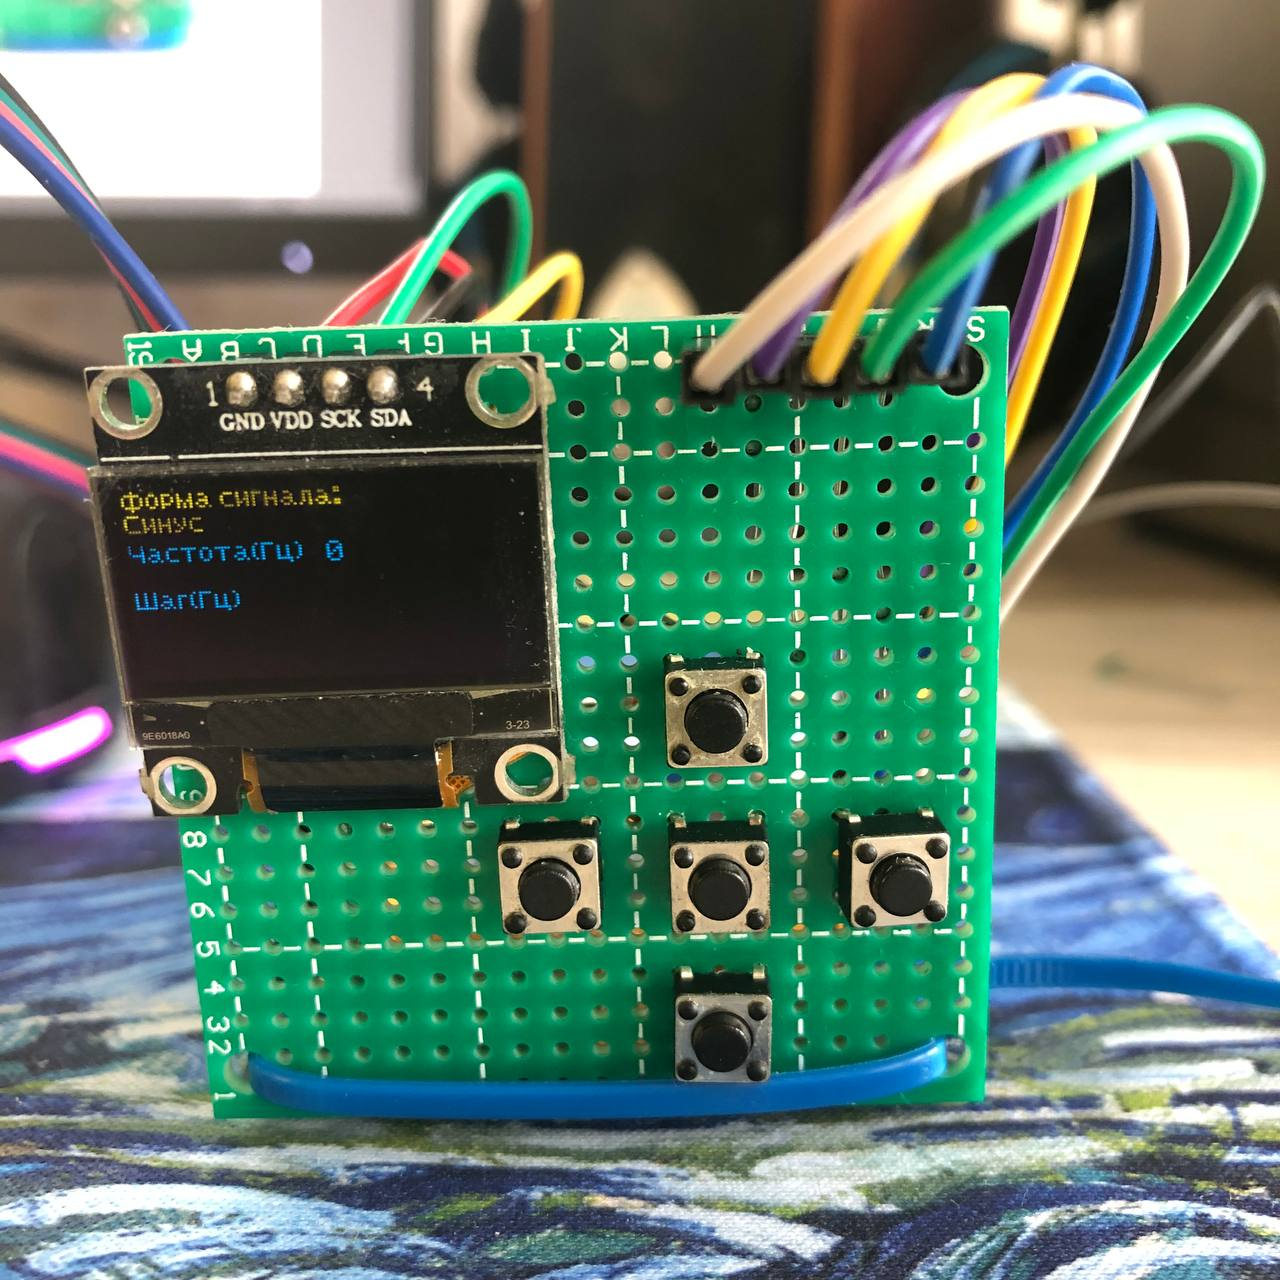
\includegraphics[width=0.9\textwidth]{../image/test1_u_s.jpg}
         \caption{Устройство.}
     \end{subfigure}
     \hfill
     \begin{subfigure}[H]{0.5\textwidth}
         \centering
         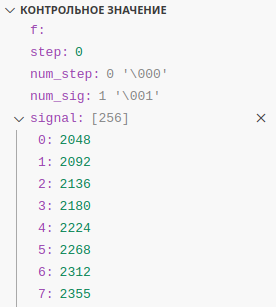
\includegraphics[width=0.8\textwidth]{../image/test1_o_s.png}
         \caption{Отладчик.}
     \end{subfigure}
        \caption{Выбор сигнала синуса.}
	\end{figure}
	
	\begin{figure}[H]
     \begin{subfigure}[H]{0.5\textwidth}
         \centering
         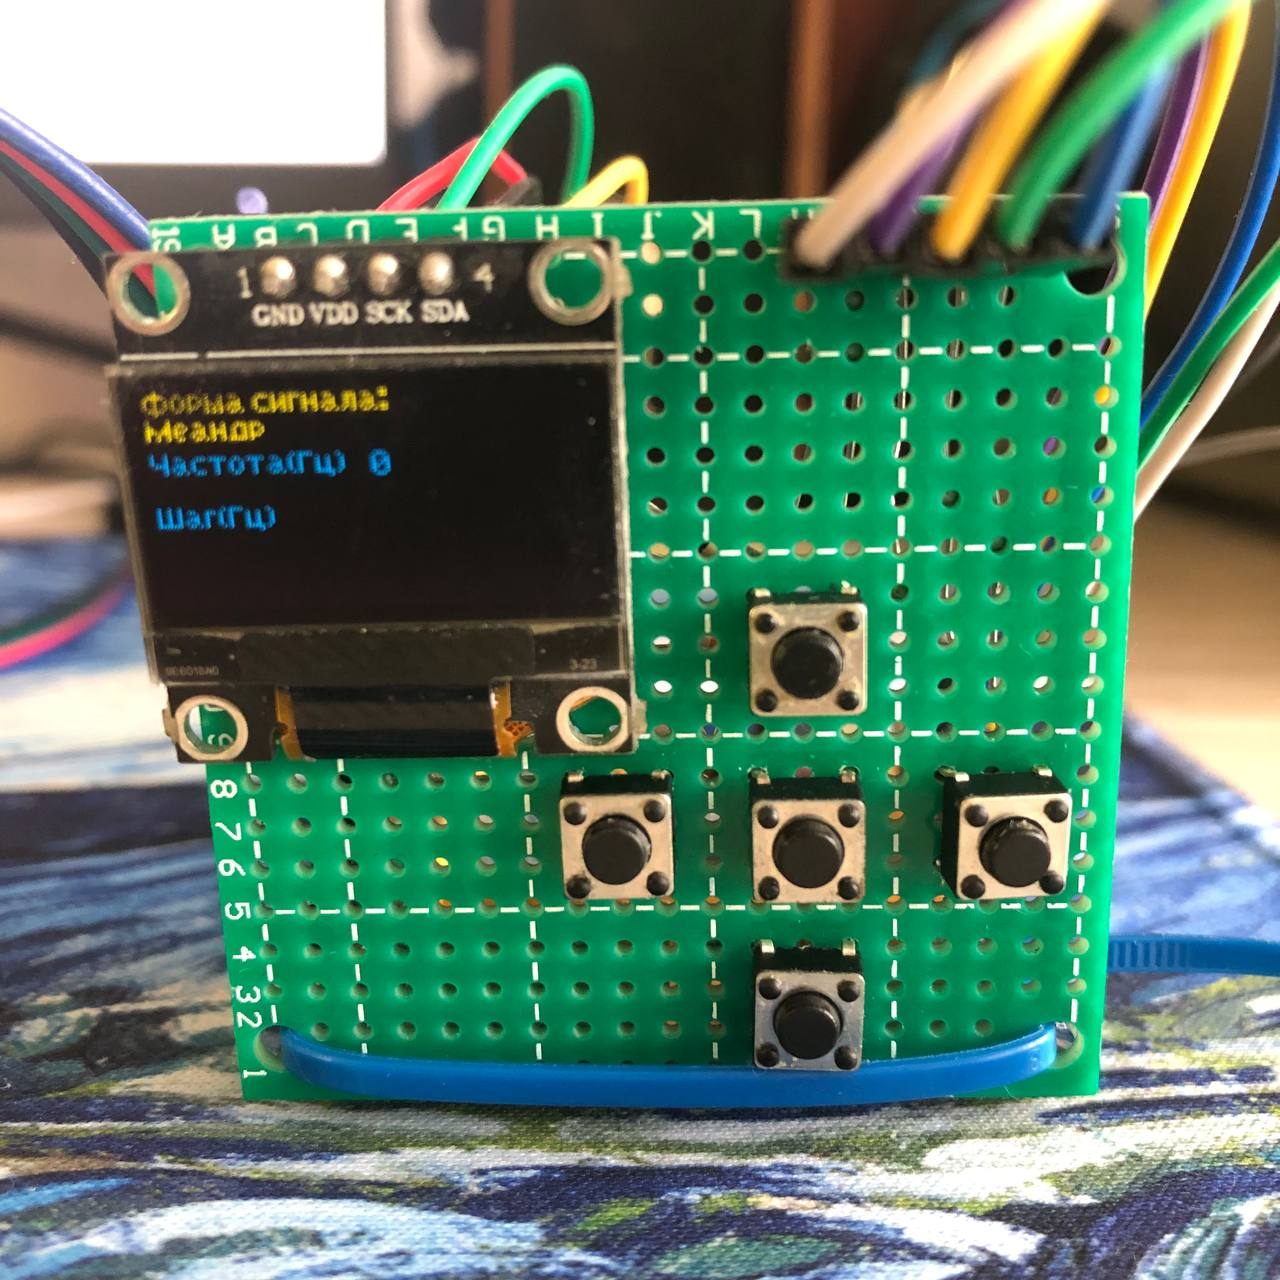
\includegraphics[width=0.9\textwidth]{../image/test2_u_s.jpg}
         \caption{Устройство.}
     \end{subfigure}
     \hfill
     \begin{subfigure}[H]{0.5\textwidth}
         \centering
         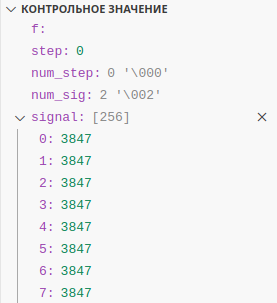
\includegraphics[width=0.8\textwidth]{../image/test2_o_s.png}
         \caption{Отладчик.}
     \end{subfigure}
        \caption{Выбор сигнала меандра.}
	\end{figure}
	
	\begin{figure}[H]
     \begin{subfigure}[H]{0.5\textwidth}
         \centering
         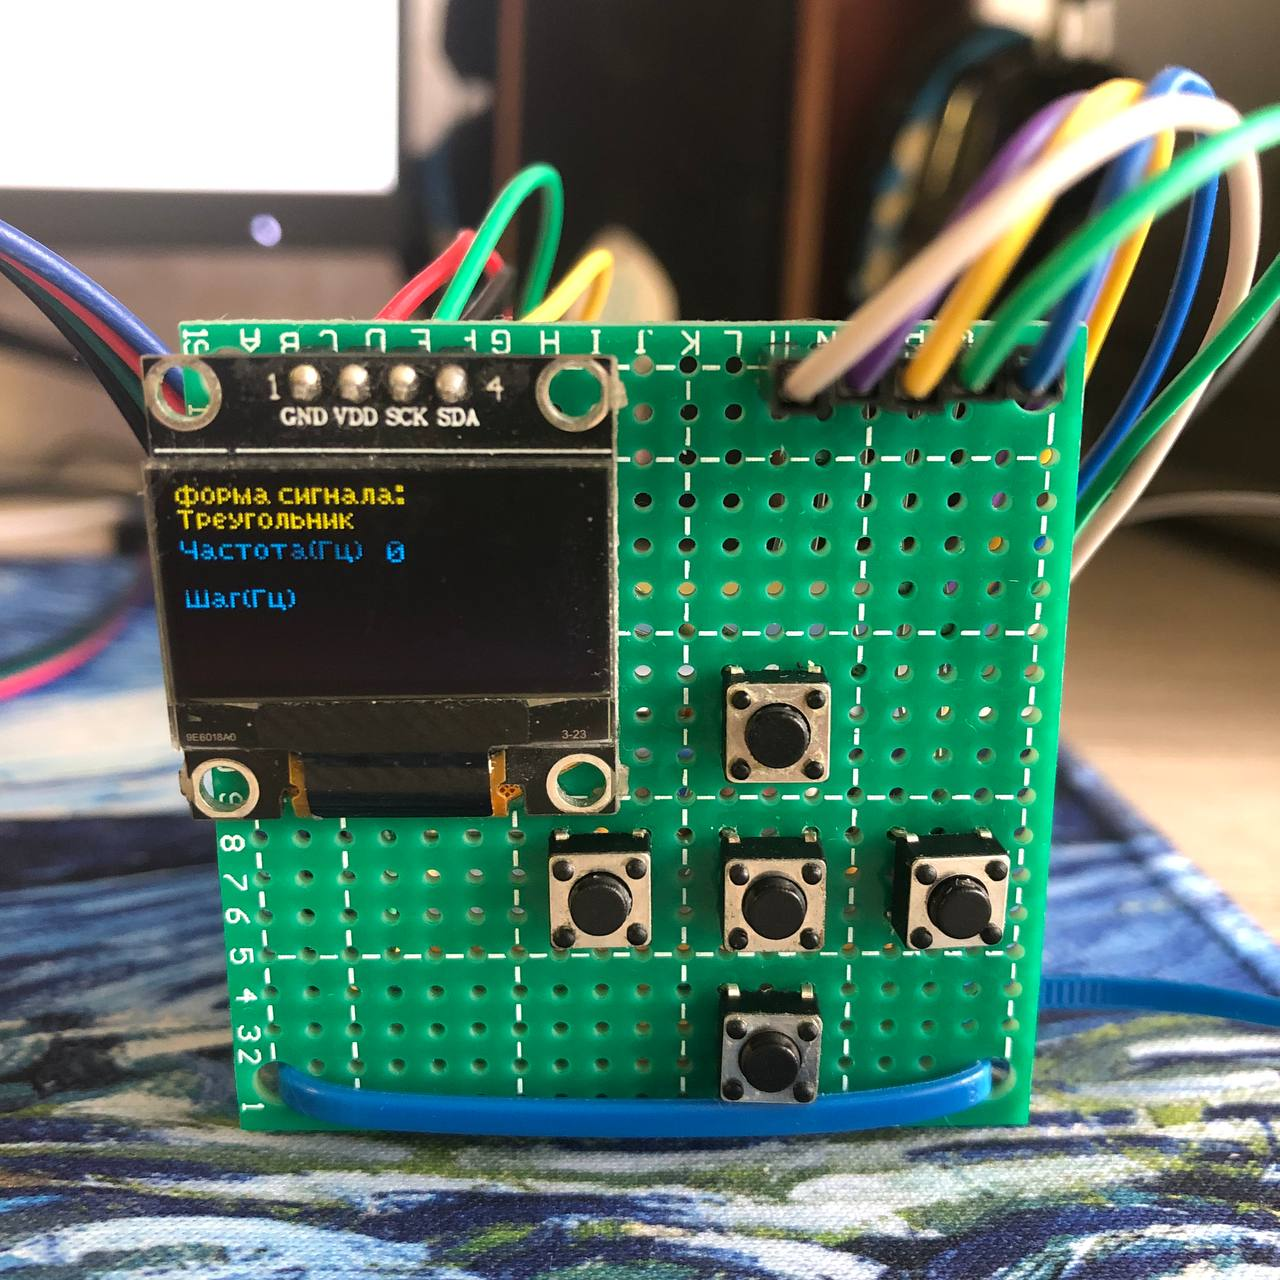
\includegraphics[width=0.9\textwidth]{../image/test3_u_s.jpg}
         \caption{Устройство.}
     \end{subfigure}
     \hfill
     \begin{subfigure}[H]{0.5\textwidth}
         \centering
         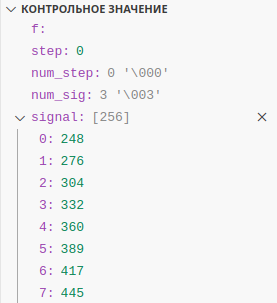
\includegraphics[width=0.8\textwidth]{../image/test3_o_s.png}
         \caption{Отладчик.}
     \end{subfigure}
        \caption{Выбор сигнала треугольника.}
	\end{figure}
	
	\begin{figure}[H]
     \begin{subfigure}[H]{0.5\textwidth}
         \centering
         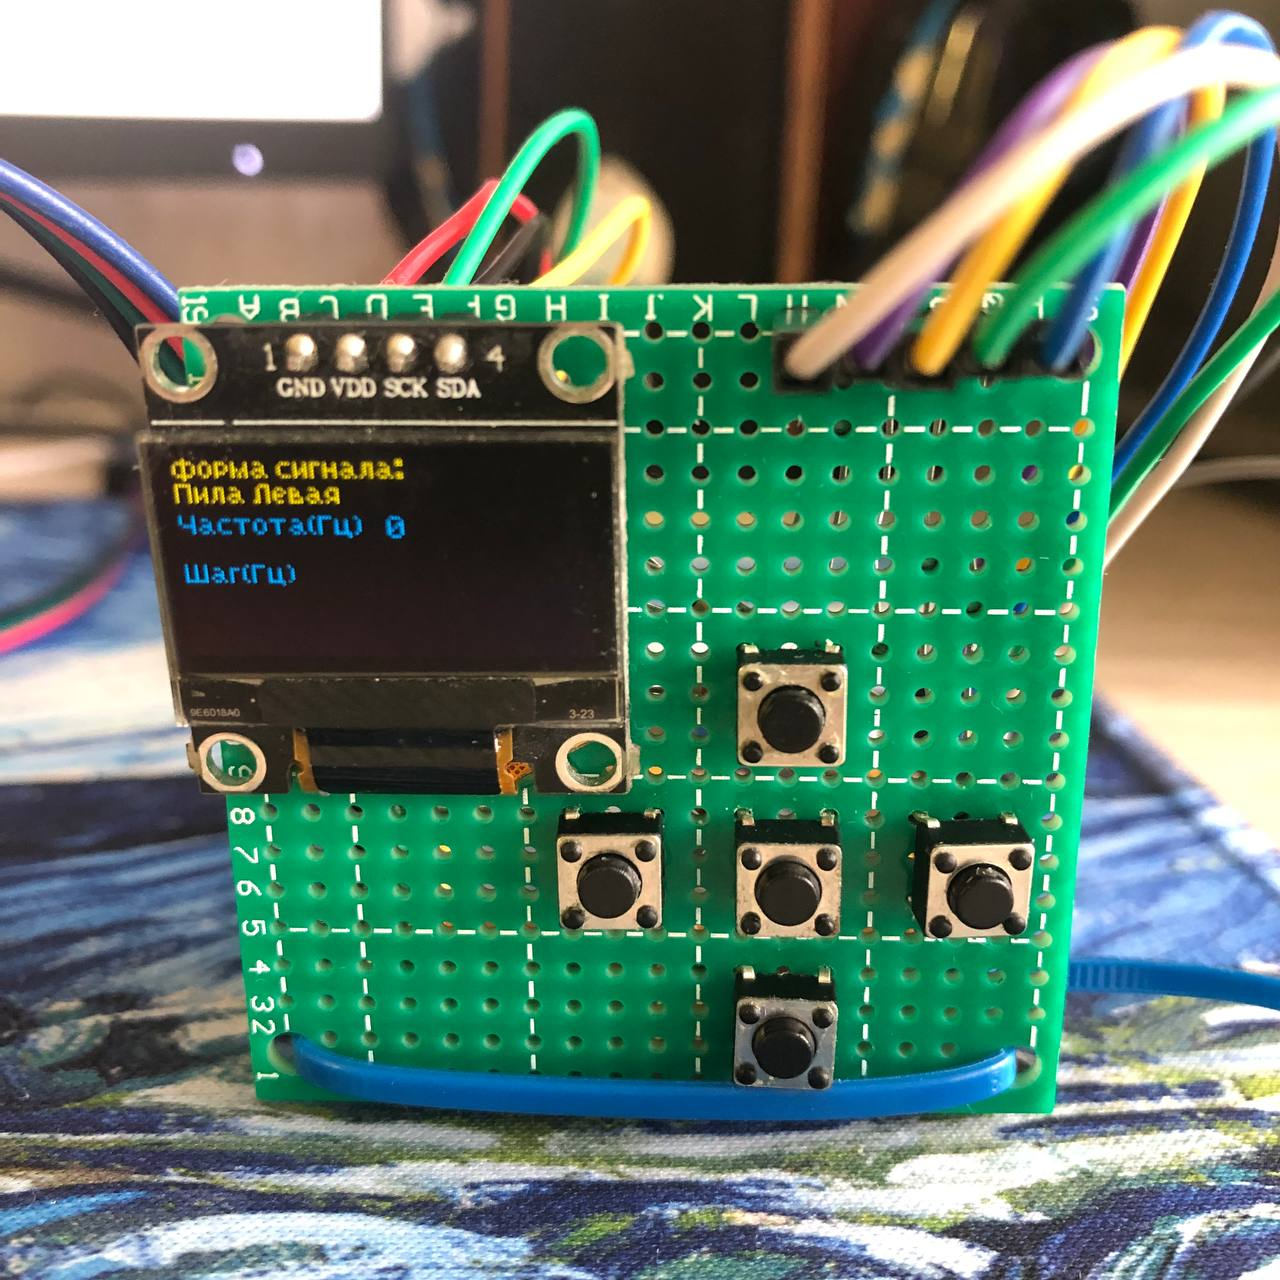
\includegraphics[width=0.9\textwidth]{../image/test4_u_s.jpg}
         \caption{Устройство.}
     \end{subfigure}
     \hfill
     \begin{subfigure}[H]{0.5\textwidth}
         \centering
         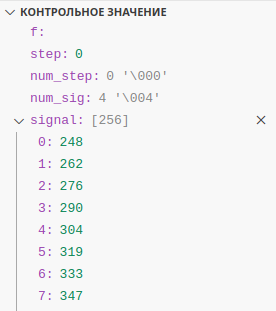
\includegraphics[width=0.8\textwidth]{../image/test4_o_s.png}
         \caption{Отладчик.}
     \end{subfigure}
        \caption{Выбор сигнала пилы левой.}
	\end{figure}
	
	\begin{figure}[H]
     \begin{subfigure}[H]{0.5\textwidth}
         \centering
         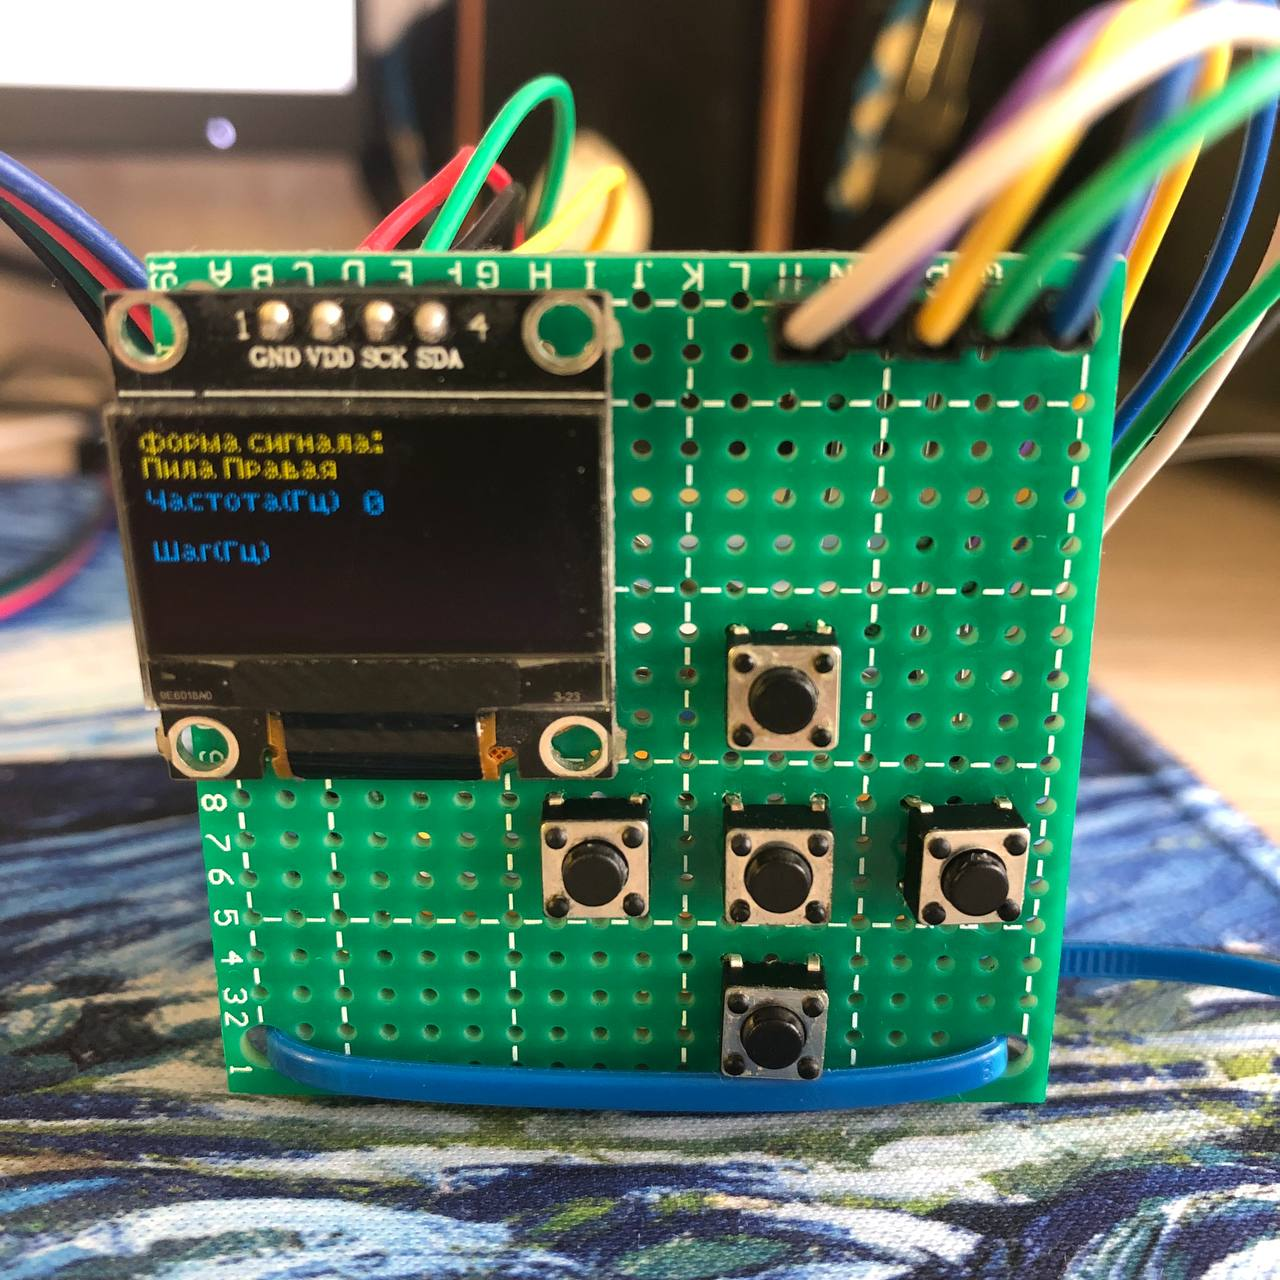
\includegraphics[width=0.9\textwidth]{../image/test5_u_s.jpg}
         \caption{Устройство.}
     \end{subfigure}
     \hfill
     \begin{subfigure}[H]{0.5\textwidth}
         \centering
         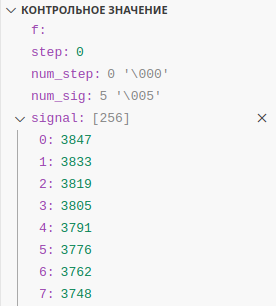
\includegraphics[width=0.8\textwidth]{../image/test5_o_s.png}
         \caption{Отладчик.}
     \end{subfigure}
        \caption{Выбор сигнала пилы правой.}
	\end{figure}
	
	Как можно заметить функция, привязанная к кнопке N выполняется корректно.

	Для клавиши P алгоритм отличается только тем, что номер сигнала нужно декрементировать. Функция также отрабатывает корректно.
	
	Теперь нужно выбрать величину шага, с которым будет регулироваться частота сигнала. Алгоритм для установки шага следующий (рис. 3.16).
	
	\begin{figure}[H]
    \centering
    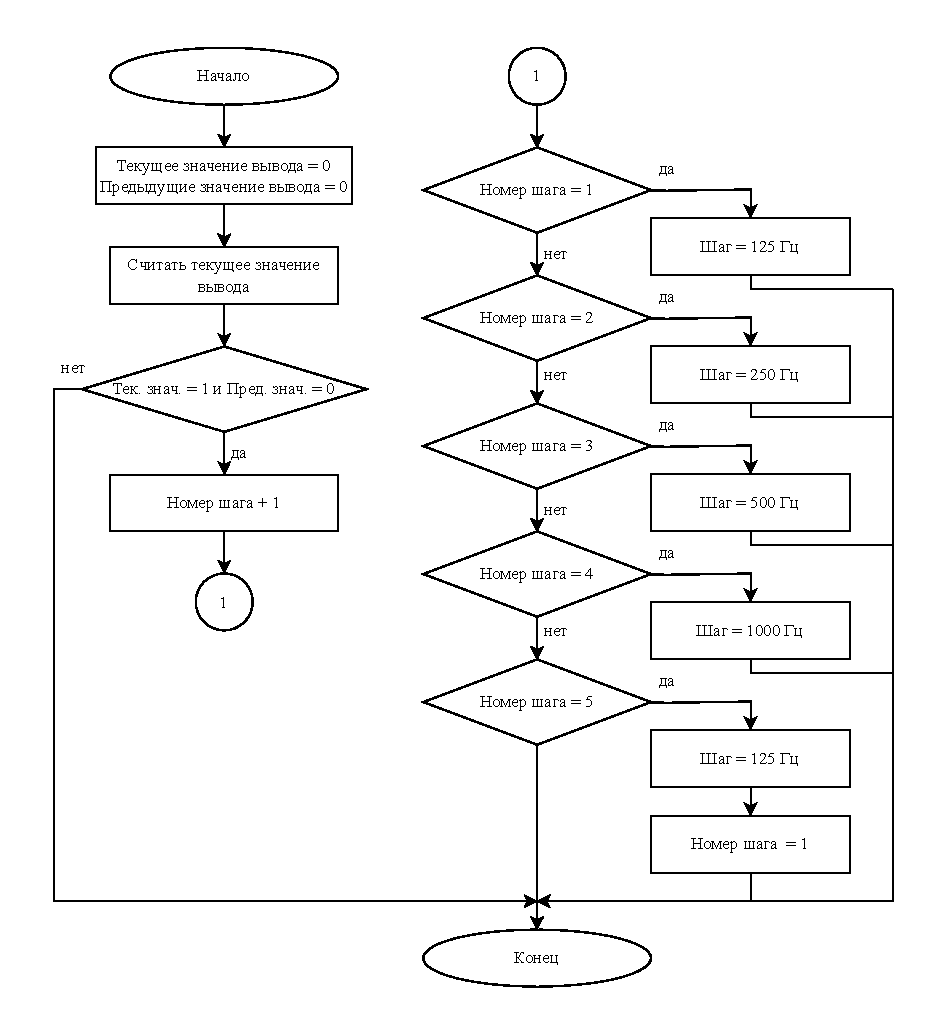
\includegraphics[width=1\textwidth]{../image/step_select.pdf}
    \caption{Выбор шага.}
	\end{figure}	
	
	
	\begin{figure}[H]
     \begin{subfigure}[H]{0.5\textwidth}
         \centering
         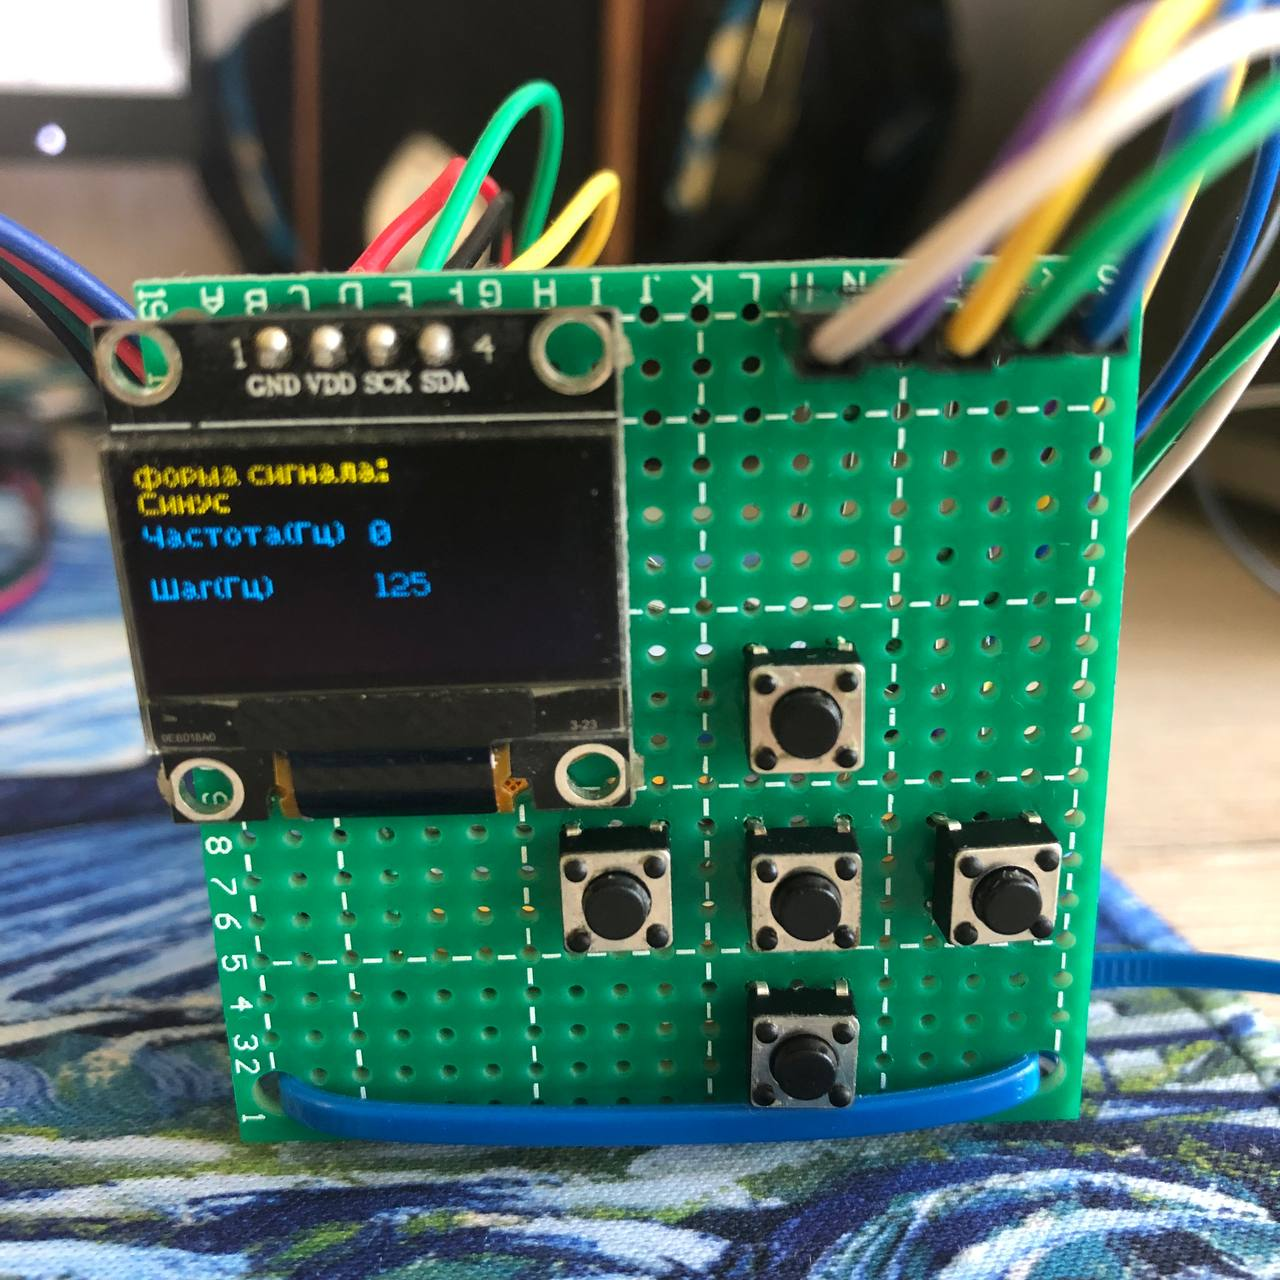
\includegraphics[width=0.9\textwidth]{../image/test1_u_st.jpg}
         \caption{Устройство.}
     \end{subfigure}
     \hfill
     \begin{subfigure}[H]{0.5\textwidth}
         \centering
         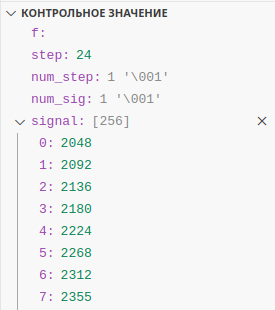
\includegraphics[width=0.8\textwidth]{../image/test1_o_st.png}
         \caption{Отладчик.}
     \end{subfigure}
        \caption{Выбор шага 125 Гц.}
	\end{figure}
	
	\begin{figure}[H]
     \begin{subfigure}[H]{0.5\textwidth}
         \centering
         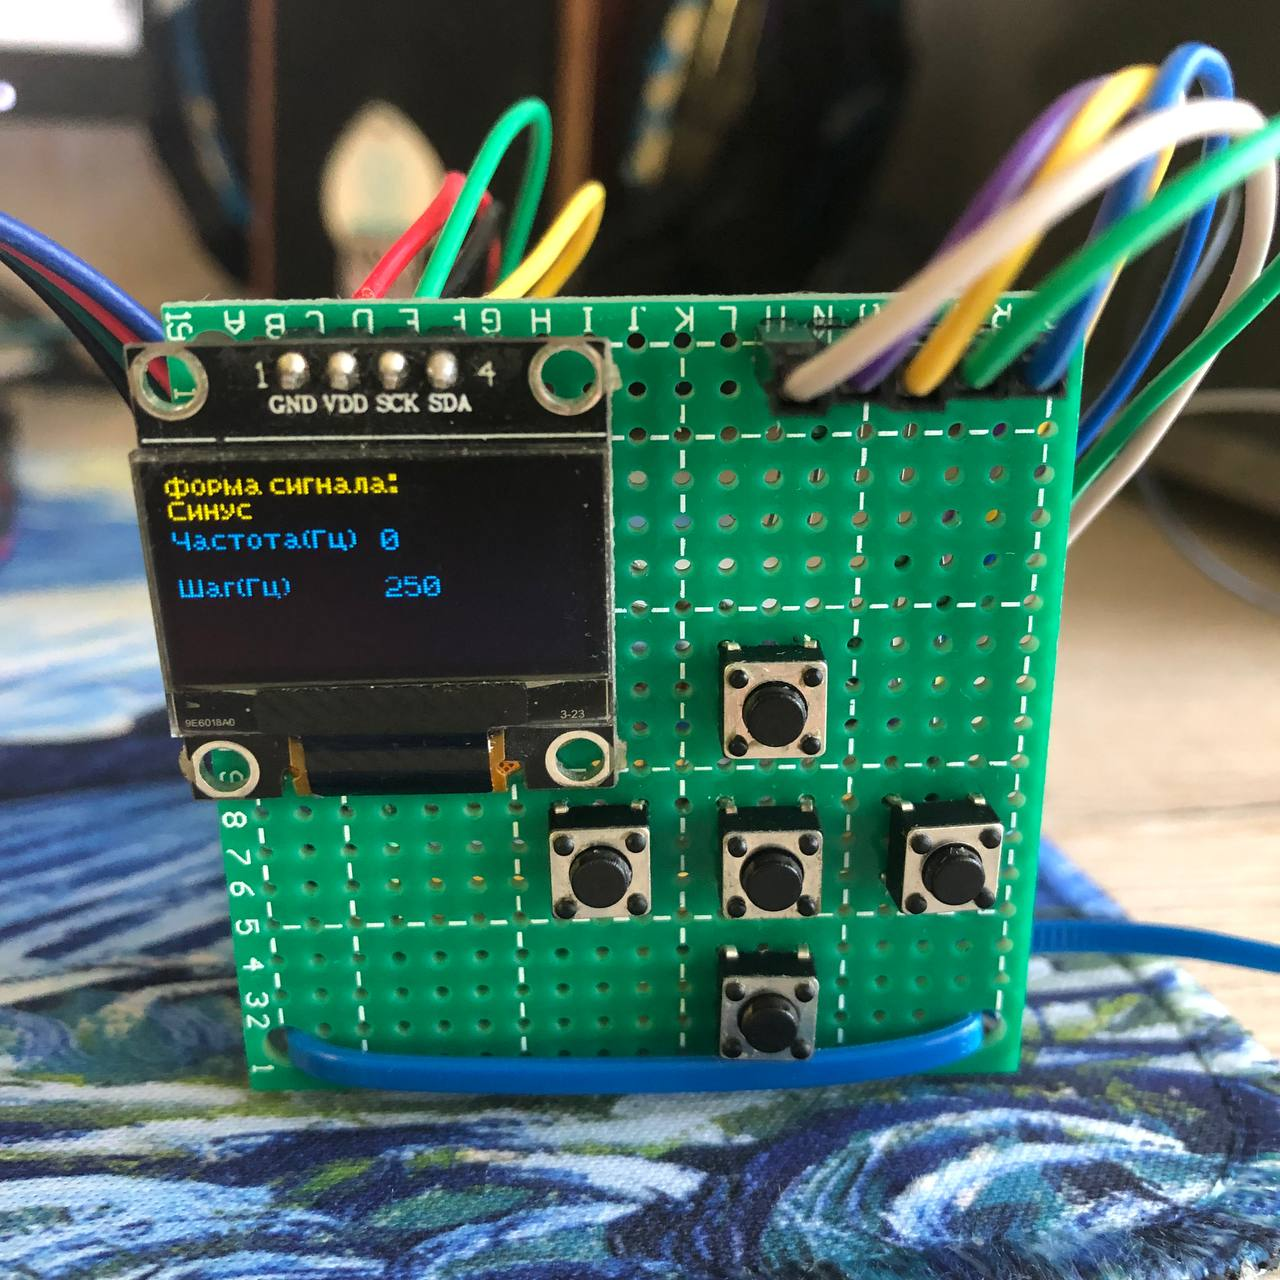
\includegraphics[width=0.9\textwidth]{../image/test2_u_st.jpg}
         \caption{Устройство.}
     \end{subfigure}
     \hfill
     \begin{subfigure}[H]{0.5\textwidth}
         \centering
         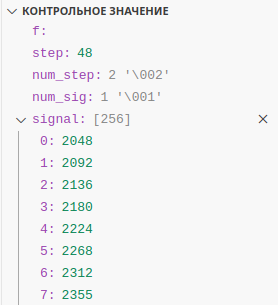
\includegraphics[width=0.8\textwidth]{../image/test2_o_st.png}
         \caption{Отладчик.}
     \end{subfigure}
        \caption{Выбор шага 250 Гц.}
	\end{figure}
	
	\begin{figure}[H]
     \begin{subfigure}[H]{0.5\textwidth}
         \centering
         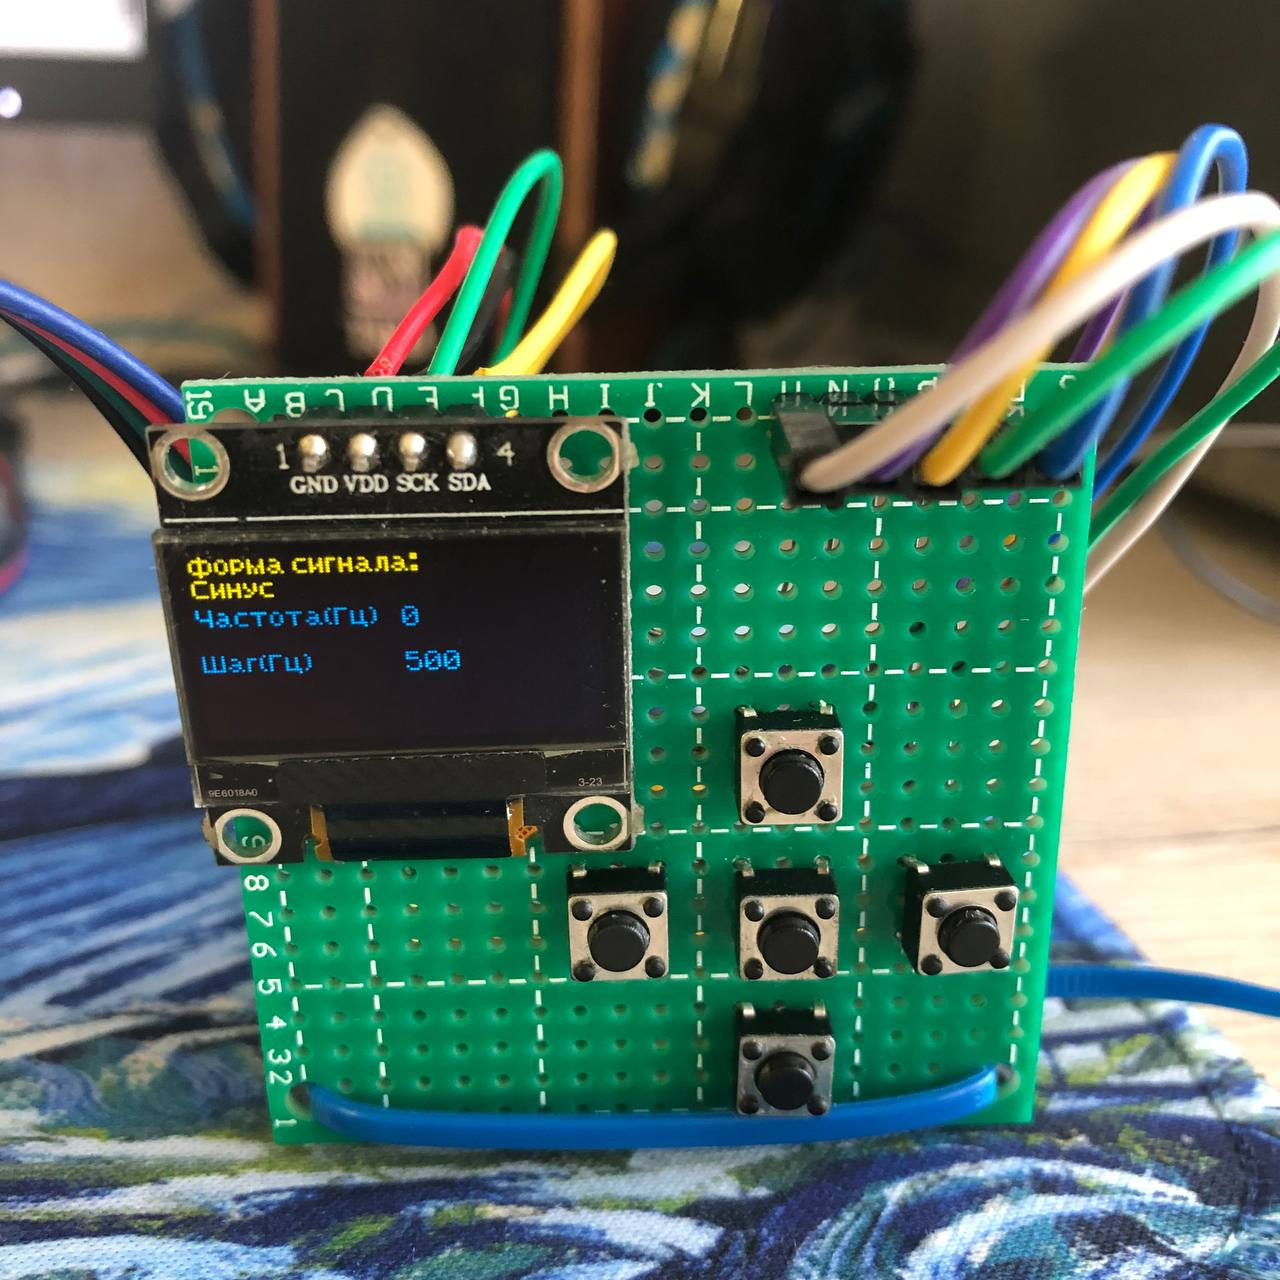
\includegraphics[width=0.9\textwidth]{../image/test3_u_st.jpg}
         \caption{Устройство.}
     \end{subfigure}
     \hfill
     \begin{subfigure}[H]{0.5\textwidth}
         \centering
         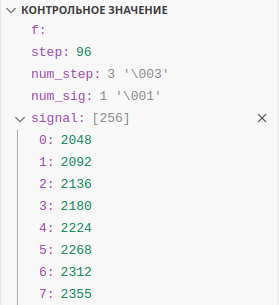
\includegraphics[width=0.8\textwidth]{../image/test3_o_st.png}
         \caption{Отладчик.}
     \end{subfigure}
        \caption{Выбор шага 500 Гц.}
	\end{figure}
	
	\begin{figure}[H]
     \begin{subfigure}[H]{0.5\textwidth}
         \centering
         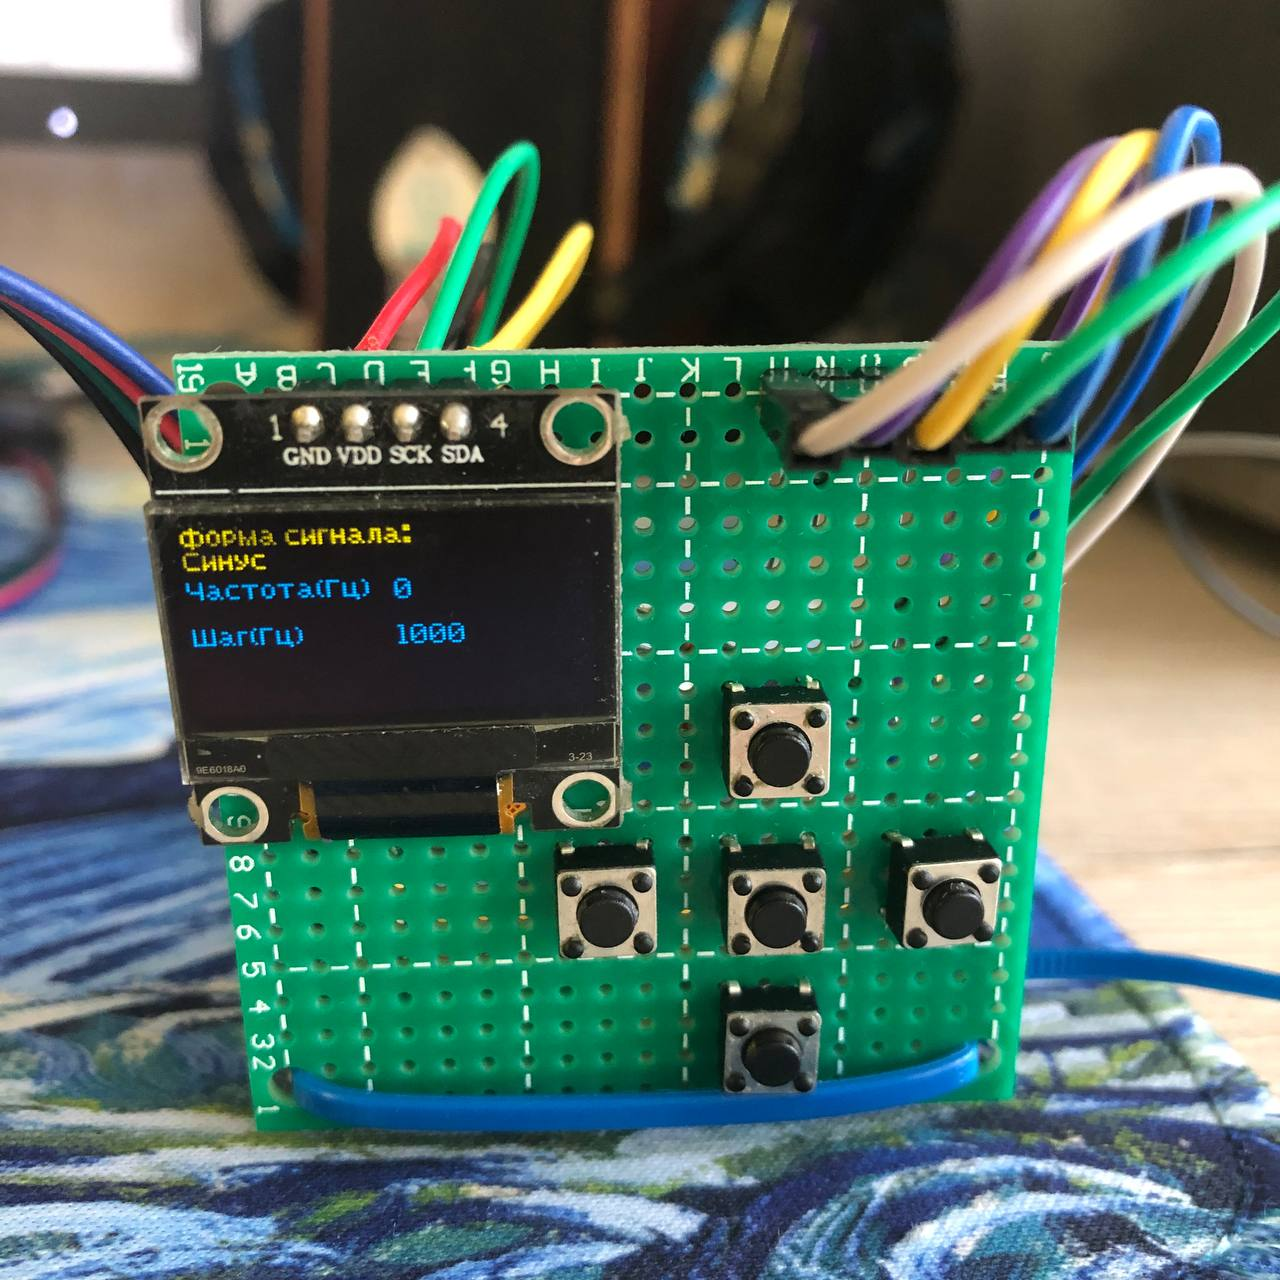
\includegraphics[width=0.9\textwidth]{../image/test4_u_st.jpg}
         \caption{Устройство.}
     \end{subfigure}
     \hfill
     \begin{subfigure}[H]{0.5\textwidth}
         \centering
         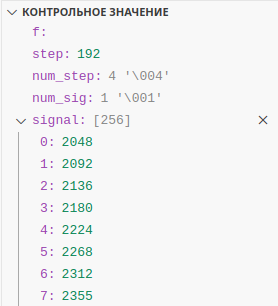
\includegraphics[width=0.8\textwidth]{../image/test4_o_st.png}
         \caption{Отладчик.}
     \end{subfigure}
        \caption{Выбор шага 1000 Гц.}
	\end{figure}
	
	Выбор шага происходит циклично, поэтому для него требуется только одна кнопка. По тестам можно сделать вывод, что функция выполняется правильно. 
	
	С помощью клавиш F- и F+ регулируется частота. Алгоритм представлен блок-схемами (рис. 3.20).
	
	\begin{figure}[H]
     \begin{subfigure}[H]{1\textwidth}
         \centering
         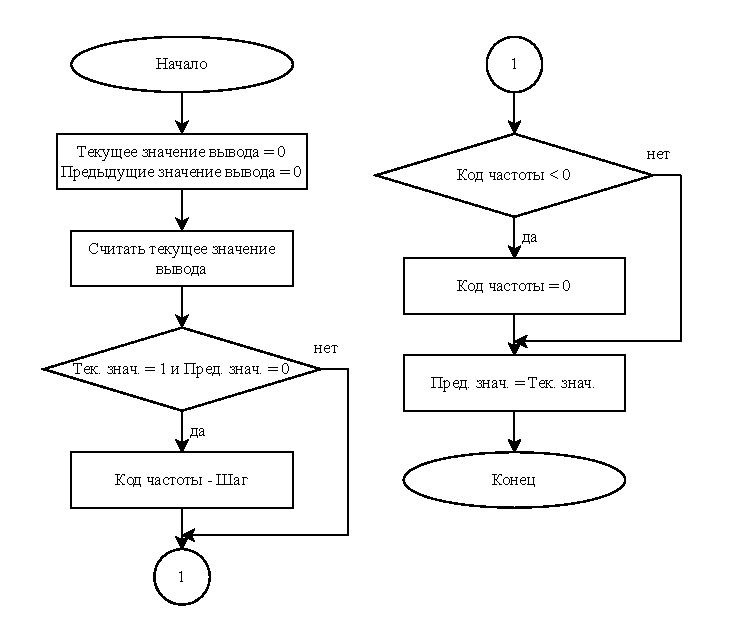
\includegraphics[width=0.775\textwidth]{../image/minus_freq.pdf}
         \caption{Уменьшение частоты.}
     \end{subfigure}
     \hfill
     \begin{subfigure}[H]{1\textwidth}
         \centering
         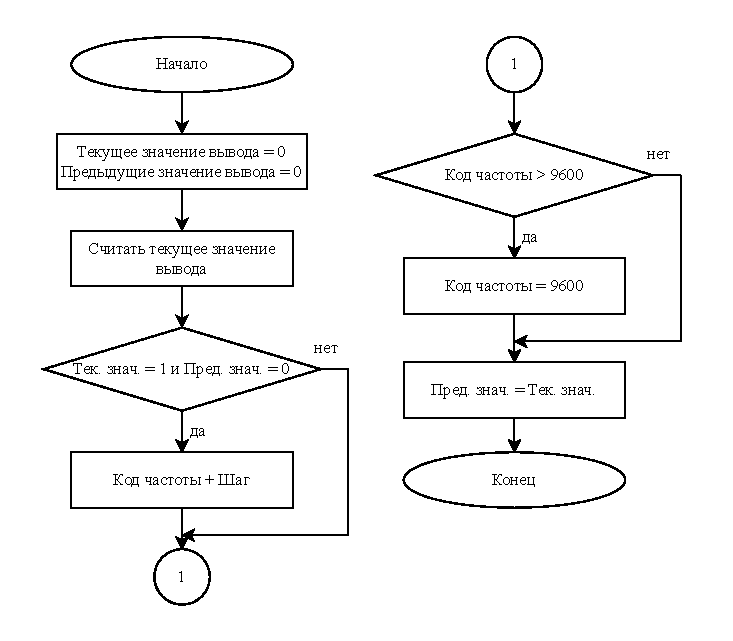
\includegraphics[width=0.775\textwidth]{../image/plus_freq.pdf}
         \caption{Увеличение частоты.}
     \end{subfigure}
        \caption{Регулировка частоты.}
	\end{figure}
	
	Проверим что расчет частоты правильный в соответствии с шагом. Частота рассчитывается по следующей формуле.
	\begin{gather}
	f = \dfrac{p_{step}}{step_{min}*f_{min}},
	\end{gather}
	
	где $p_{step}$ --- текущий код частоты,
	
	$step_{min}$ --- минимальный код частоты,
	
	$f_{min}$ --- минимальный шаг по частоте.
	
	\begin{figure}[H]
     \begin{subfigure}[H]{0.5\textwidth}
         \centering
         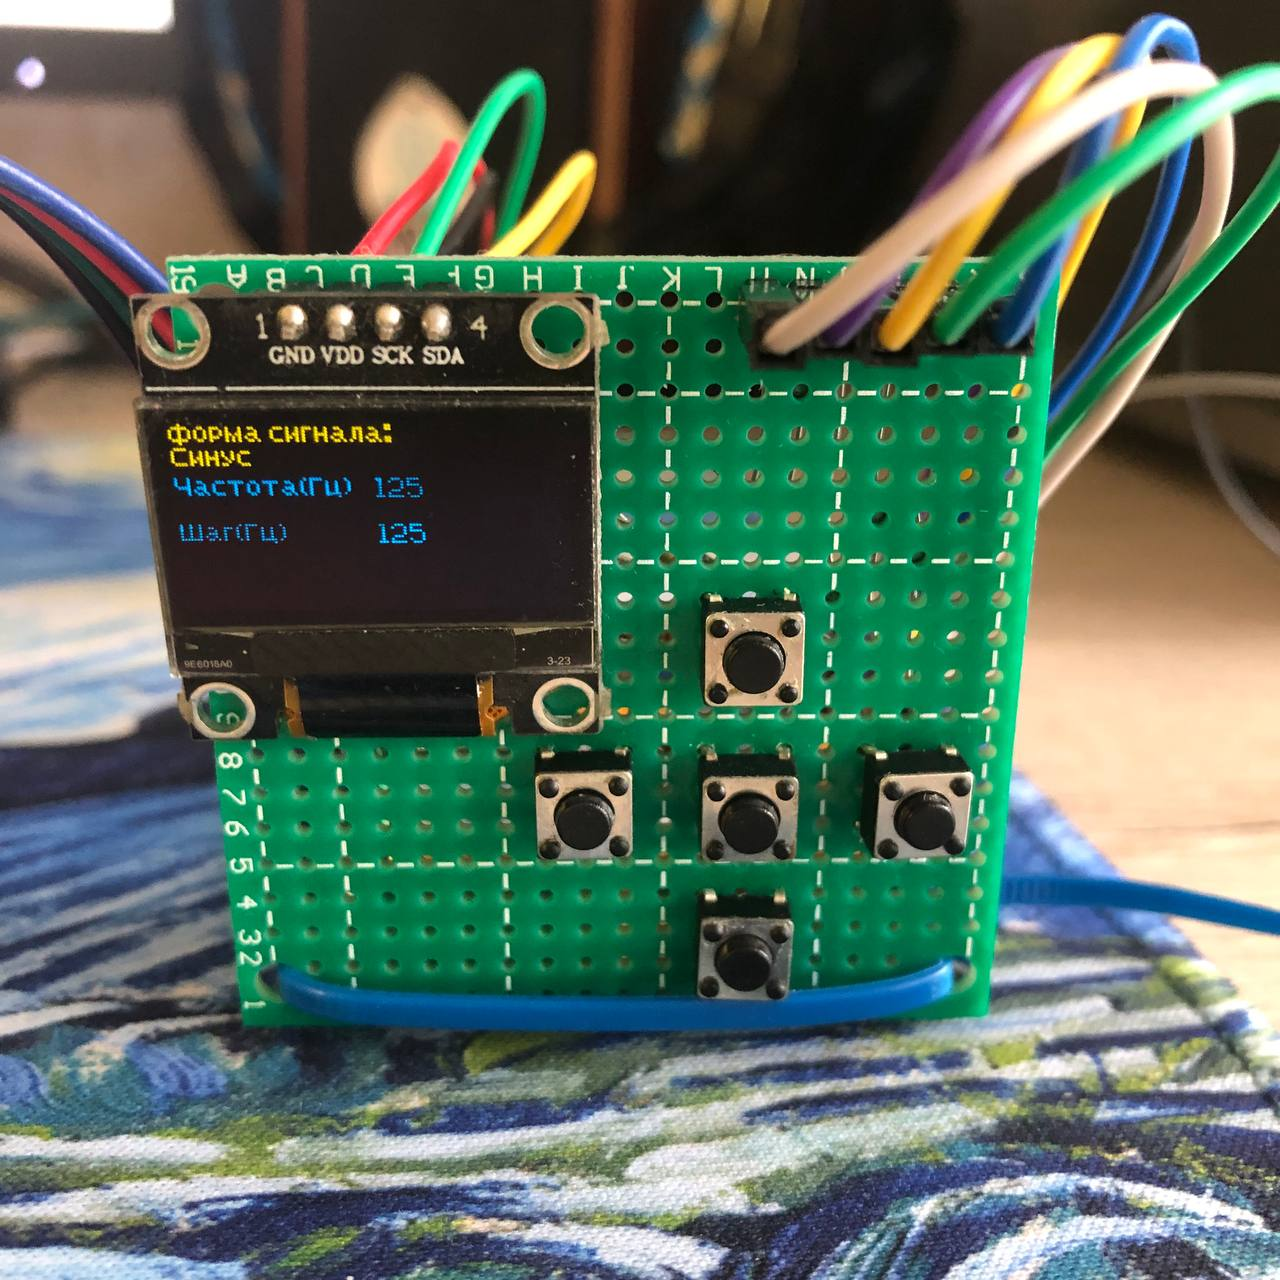
\includegraphics[width=0.8\textwidth]{../image/test1_u_f.jpg}
         \caption{Устройство.}
     \end{subfigure}
     \hfill
     \begin{subfigure}[H]{0.5\textwidth}
         \centering
         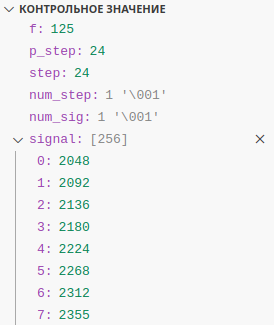
\includegraphics[width=0.7\textwidth]{../image/test1_o_f.png}
         \caption{Отладчик.}
     \end{subfigure}
        \caption{Шаг 125 Гц.}
	\end{figure}
	
	\begin{figure}[H]
     \begin{subfigure}[H]{0.5\textwidth}
         \centering
         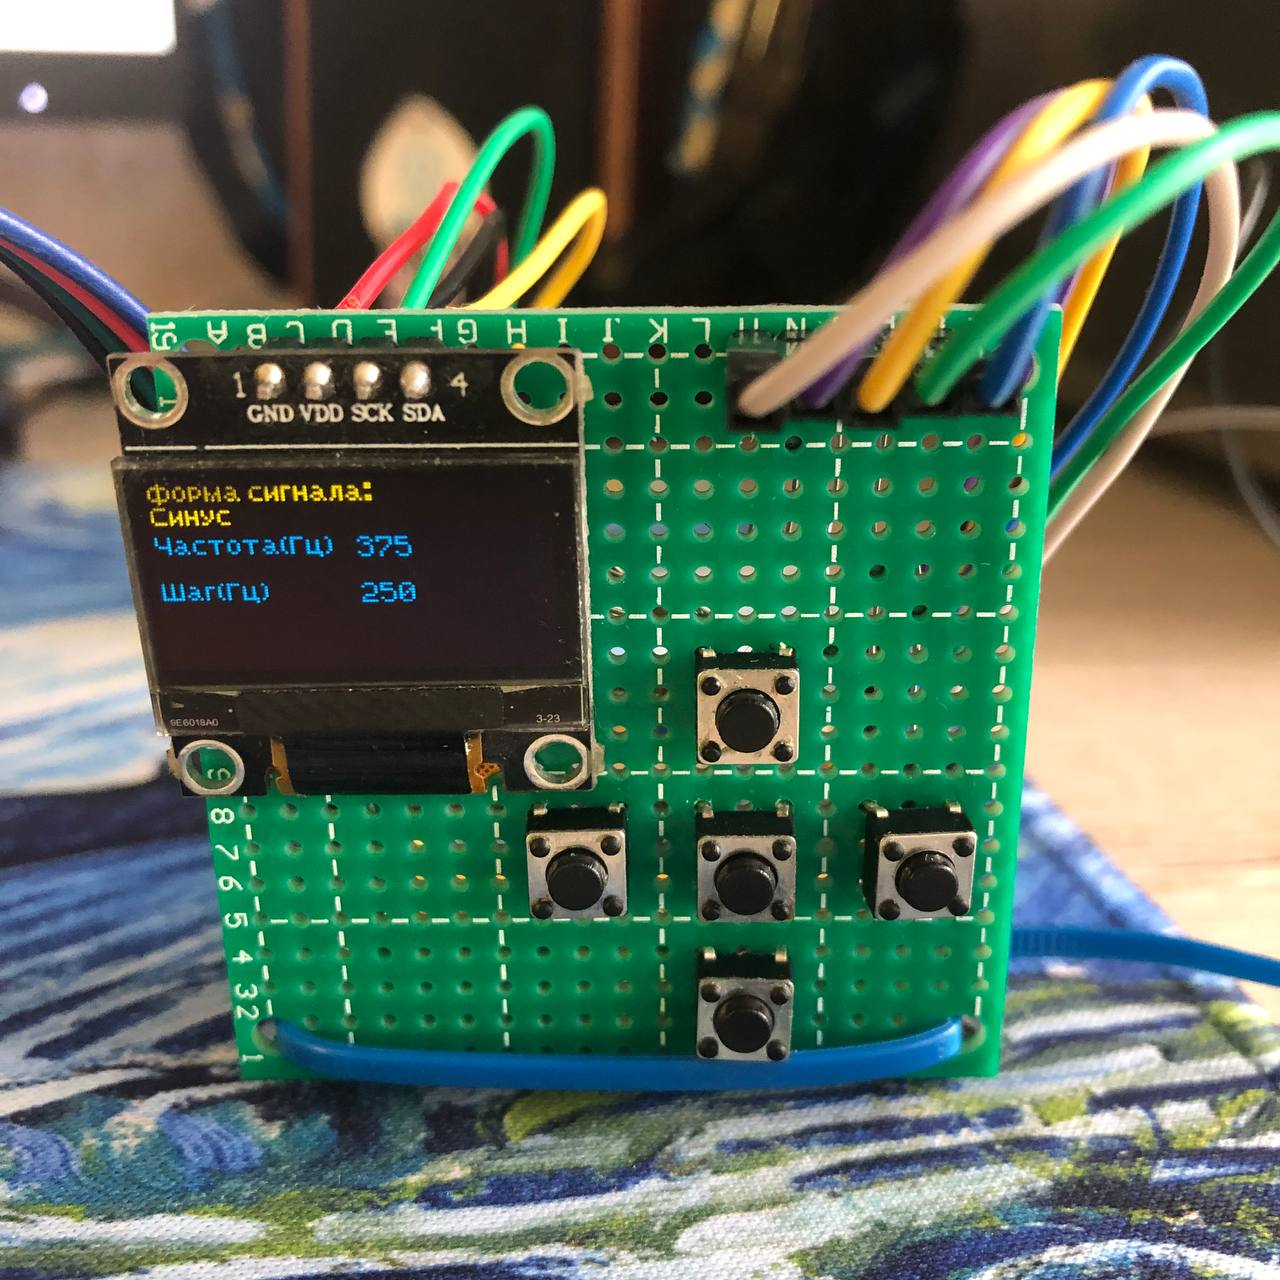
\includegraphics[width=0.8\textwidth]{../image/test2_u_f.jpg}
         \caption{Устройство.}
     \end{subfigure}
     \hfill
     \begin{subfigure}[H]{0.5\textwidth}
         \centering
         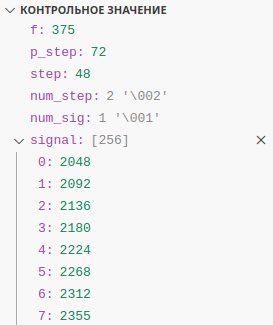
\includegraphics[width=0.7\textwidth]{../image/test2_o_f.png}
         \caption{Отладчик.}
     \end{subfigure}
        \caption{Шаг 250 Гц.}
	\end{figure}
	
	\begin{figure}[H]
     \begin{subfigure}[H]{0.5\textwidth}
         \centering
         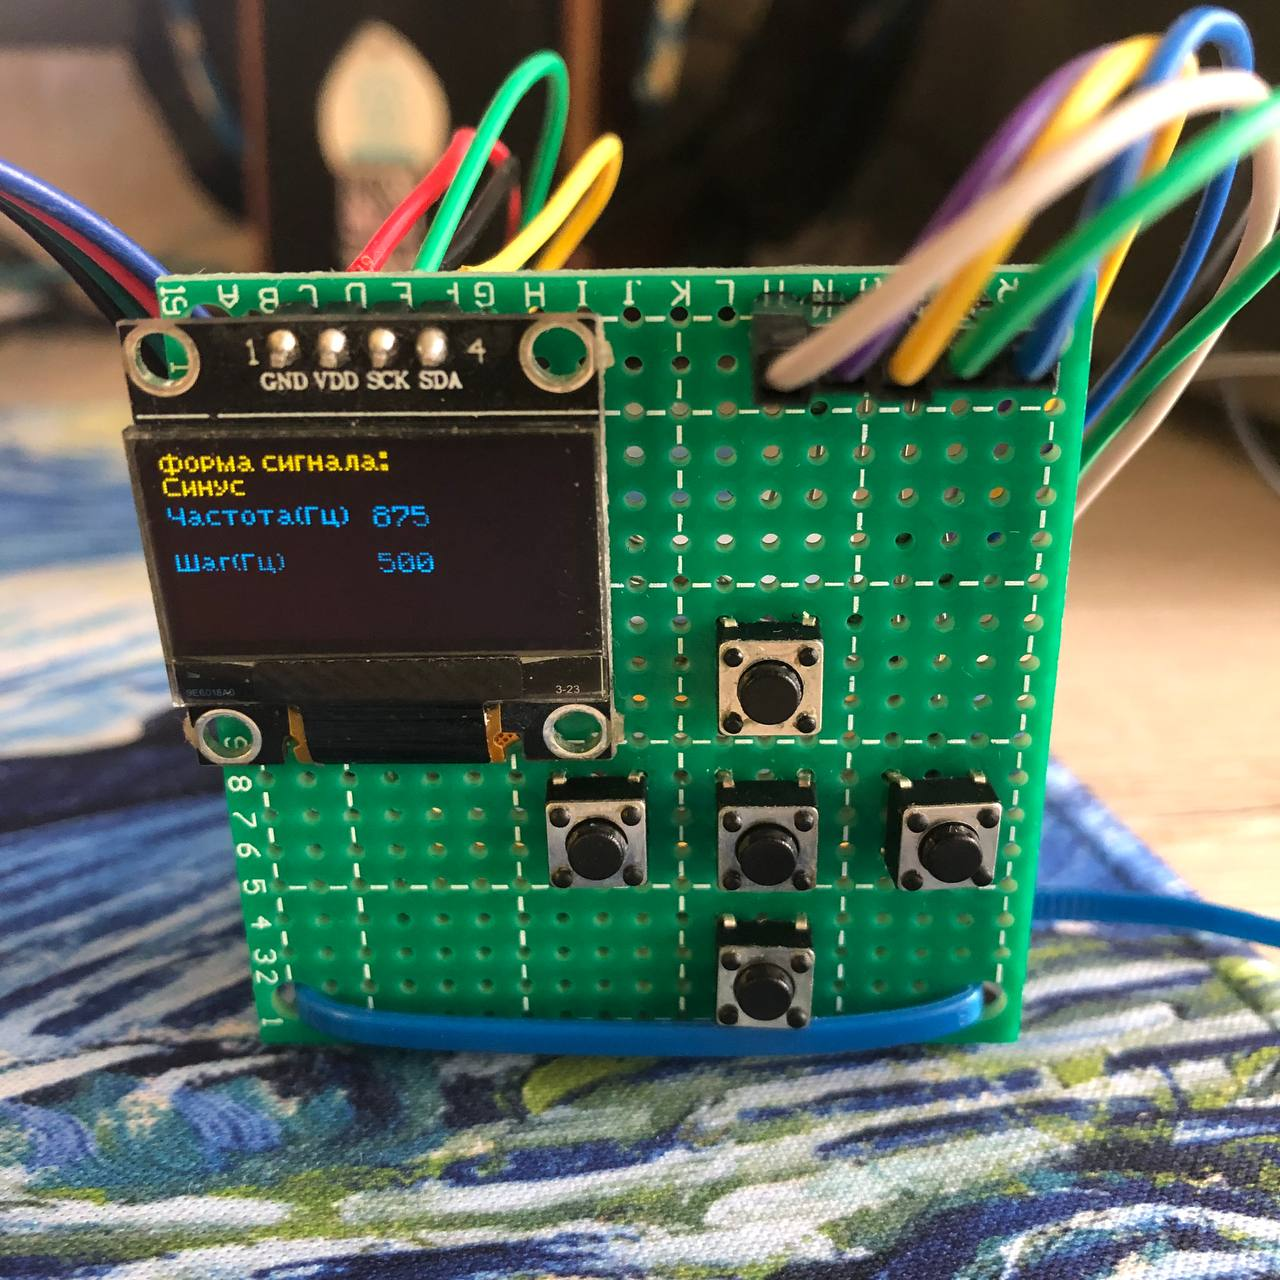
\includegraphics[width=0.9\textwidth]{../image/test3_u_f.jpg}
         \caption{Устройство.}
     \end{subfigure}
     \hfill
     \begin{subfigure}[H]{0.5\textwidth}
         \centering
         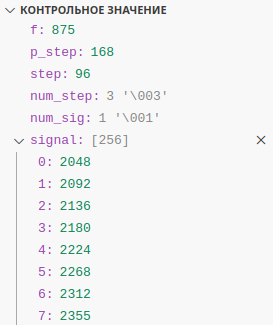
\includegraphics[width=0.8\textwidth]{../image/test3_o_f.png}
         \caption{Отладчик.}
     \end{subfigure}
        \caption{Шаг 500 Гц.}
	\end{figure}
	
	\begin{figure}[H]
     \begin{subfigure}[H]{0.5\textwidth}
         \centering
         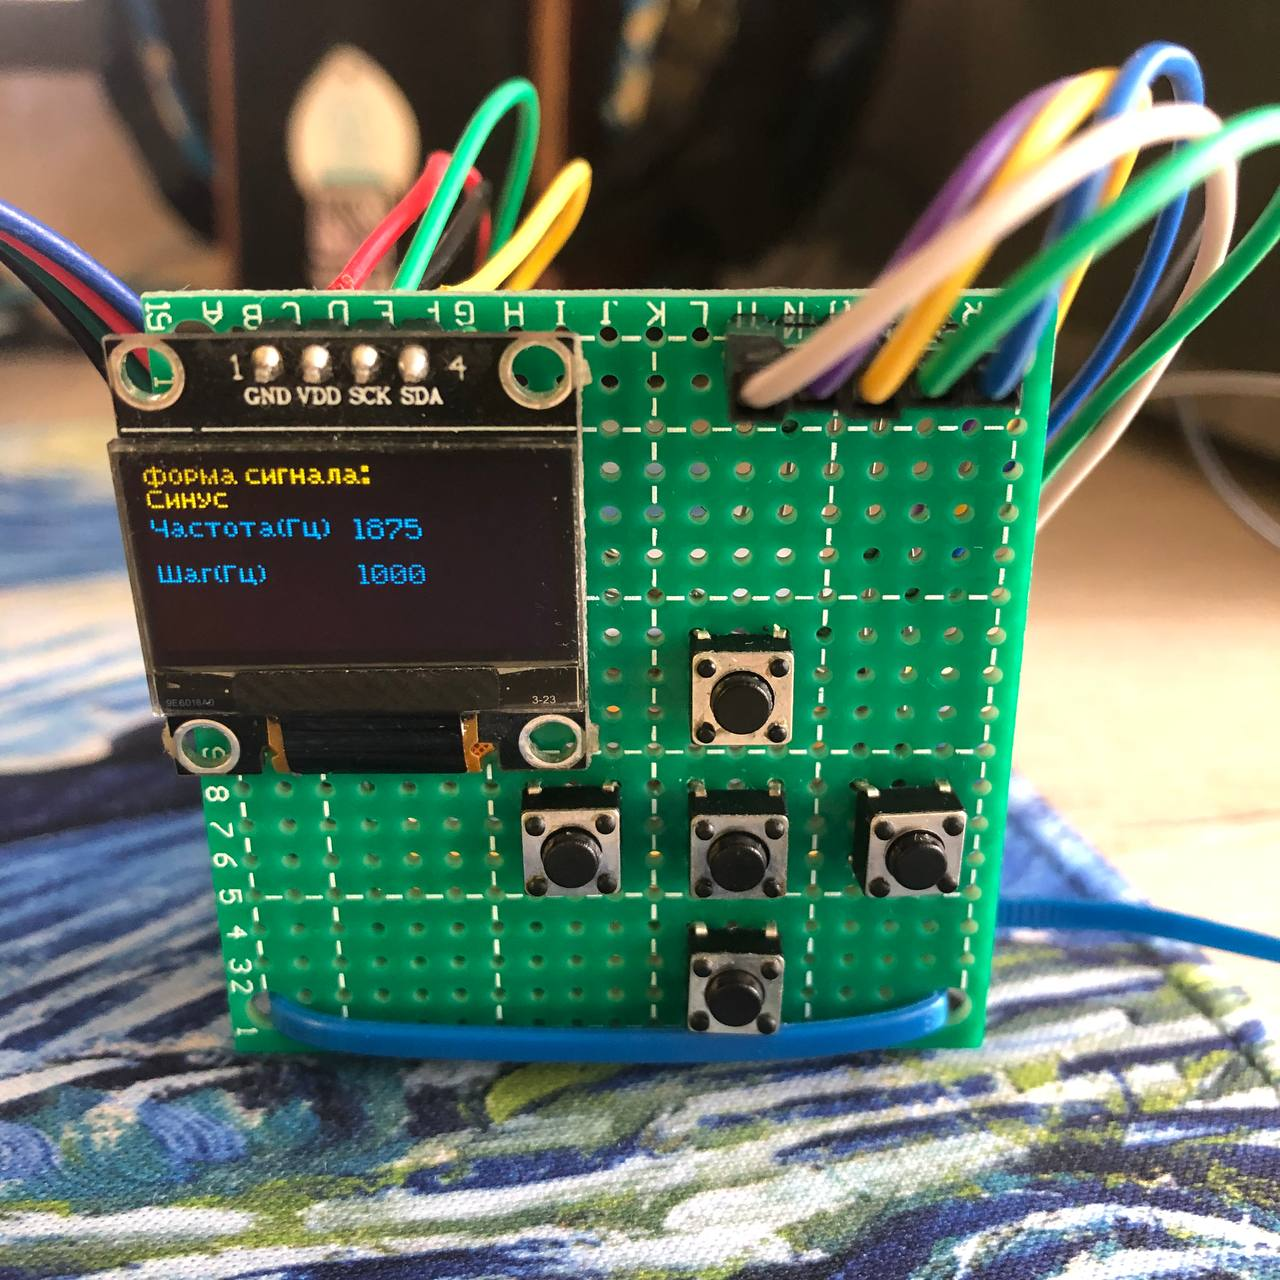
\includegraphics[width=0.9\textwidth]{../image/test4_u_f.jpg}
         \caption{Устройство.}
     \end{subfigure}
     \hfill
     \begin{subfigure}[H]{0.5\textwidth}
         \centering
         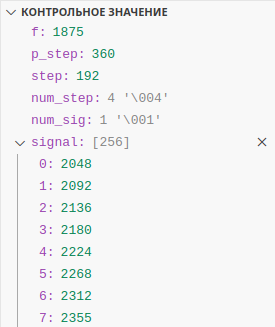
\includegraphics[width=0.8\textwidth]{../image/test4_o_f.png}
         \caption{Отладчик.}
     \end{subfigure}
        \caption{Шаг 1000 Гц.}
	\end{figure}
	
	В соответствии с частотами сделаем осциллограммы todo.
	
\section{Вывод из третьей главы}
